
\cleartoverso 
\chaptercontents{Homological Algebra}{homologicalcover.tex}{These notes are meant as a quick reference guide for the constructions in homological algebra that we will use throughout the course, and are not in any way suppose to be a substitute for a proper set of notes on homological algebra.}
\label{chap:homologicalalgebra}

\begin{elevator}[Vector Spaces, Sets, and Diagrams]
	Before we start with the development of homological algebra, it is a good idea to set up some common conventions and diagrams for simplifying linear algebra. 
\end{elevator}

\label{sec:chaincomplexes:intro}
%We've already developed some of these tools independently in \ref{sec:graph:cyclespace}, but
These are some class notes! Please lets me if you know see any errors. Here we will flesh these methods out in more detail before developing chain complexes. \\
\begin{definition}[Direct Sum]
Let $V_1$ and $V_2$ be vector spaces. The \emph{direct sum} of $V_1$ and $V_2$ is the vector space of pairs of vectors, and is denoted 
\[V_1\oplus V_2:=\{(v_1, v_2)\;|\; v_1\in V_1, v_2\in V_2\}.\]
\end{definition}
The vector addition on $V_1\oplus V_2$ is done component wise,
\[(v_1, v_2)+(w_1, w_2)=(v_1+w_1, v_2+w_2).\]
The scalar multiplication acts on all components simultaneously,
\[\lambda\cdot (v_1, v_2)= (\lambda\cdot v_1, \lambda\cdot v_2).\]
\begin{example}[Real $n$ dimensional space]
	The set of $n$-tuples of real numbers is usually denoted $\RR^n$. Another way of presenting this vector space is 
	\[\RR^n=\underbrace{\RR\oplus \RR \oplus \cdots \oplus \RR\oplus \RR}_n\]
	where now each ``vector'' $r_i\in R^1_i$ is a scalar. 
	\end{example}
The direct sum operation is commutative, in that the vector spaces $V_1\oplus V_2$ is isomorphic to $V_2\oplus V_1$. Additionally, the direct sum of vector spaces is an associative operation so that the vector spaces $(V_1\oplus V_2)\oplus V_3$ is isomorphic to $V_1\oplus(V_2\oplus V_3)$. 
If this looks suspiciously like addition on the integers to you, you're picking up on an intertwining between these two operations via dimension:
\[\dim(V_1\oplus V_2)=\dim(V_1)+ \dim(V_2.)\]
\begin{example}The rank nullity theorem can be restated as: If $f: V\to W$ is a linear map, then 
\[V\simeq \ker f\oplus \im f. \]
\end{example}
Given vector spaces $V_1, V_2, W$, and maps $f_1: V_1\to W$, $f_2: V_2\to W$, one can create a new map from $V_1\oplus V_2\to W$, which is defined by taking the sum of the two maps:
\begin{align*}
f_1\oplus f_2: V_1\oplus V_2 \to&  W\\
(v_1, v_2)\mapsto& f_1(v_1)+f_2(v_2).
\end{align*}
We will frequently represent this composition either \emph{diagrammatically} or {using matrices.}
This is a useful shorthand, and we will use it throughout this section on chain complexes.

\[
\begin{tikzcd}
V_1\arrow{dr}{f_1}\\
\oplus & W\\
V_2 \arrow{ur}{f_2}
\end{tikzcd}
\;\;\;\;\;\begin{pmatrix} f_1 & f_2 \end{pmatrix} \cdot \begin{pmatrix} v_1\\v_2\end{pmatrix} = \begin{pmatrix}f_1(v_1)+f_2(v_2) \end{pmatrix}.
\]
There is nothing that limits us to taking the direct sum of more than one map along the domain. 
\begin{definition}[Sum across common target]
Let $f_i: V_i\to W$ be a collection of maps. Then define $\bigoplus_{i=1}^k f_i: \bigoplus_{i=1}^k V_i\to W$ be the map defined on tuples by
\[\left(\bigoplus f_i\right)(v_1, \ldots, v_{k})=\sum_{i=1}^k f_i(v_i).\]
\end{definition}
Just as we can take the sum along the domains of maps, we are also allowed to take sums along the targets of the maps. 
Let $g_1: V\to W_1$ and $g_2: V\to W_2$ be two linear maps. Then denote the direct sum along the target
\begin{align*}
g_1\oplus g_2: V\to & W_1\oplus W_2\\
v\mapsto& (g_1(v), g_2(v).)
\end{align*}
Just as we did for direct sum along the domain, we can represent these maps diagrammatically or with matrices. 
\[\begin{tikzcd}
\;& W_1\\
V\arrow{ur}{g_1}   \arrow{dr}{g_2} & \oplus \\
\; & W_2 
\end{tikzcd}\;\;\;\;\;\;\;\;\;\;\;\;\begin{pmatrix} g_1 \\ g_2 \end{pmatrix} \cdot \begin{pmatrix} v\end{pmatrix} = \begin{pmatrix}g_1(v_1)\\g_2(v_2) \end{pmatrix}.\]
We can quickly do this with many targets at the same time.
\begin{definition}[Sum across common domain]
Let $g_i: V\to W_i$ be a collection of linear maps. Define their direct sum to be 
\begin{align*}
\bigoplus_{i=1}^k g_i: V\to& \bigoplus_{i=1}^k W_i\\
v\mapsto& (g_1(v), g_2(v) \cdots , g_k(v)).
\end{align*}
\end{definition}
By combining both processes, we can create maps from many domains and targets simultaneously. 
\begin{definition}[Sum across domains and targets]
Let $f_{ij}: V_i\to W_j$ be a collection of linear maps. Define their direct sum to be 
\begin{align*}
\bigoplus_{i,j} f_{ij}: \bigoplus_{i=1}^m V_i\to\bigoplus_{j=1}^n W_j\\
(v_1, \ldots, v_m)\mapsto & \left(\sum_{i=1}^mf_{i,1}(v_i), \sum_{i=1}^mf_{i,2}(v_i), \ldots, \sum_{i=1}^mf_{i,{n-1}}(v_i), \sum_{i=1}^mf_{i,{n}}(v_i)\right).
\end{align*}
\end{definition}
We again have diagrammatic and matrix notations for these maps. 
\[
\begin{tikzcd}[row sep= tiny]
V_1\arrow{r} \arrow{rdd}  & W_1\\
\oplus & \oplus \\
V_2\arrow{r}  \arrow{ruu} & W_2
\end{tikzcd}\;\;\;\;\;\;\;\;\;\;\;\;
\begin{pmatrix}
f_{11}& f_{21}\\f_{12} & f_{22}
\end{pmatrix}
\begin{pmatrix} v_1 \\ v_2\end{pmatrix} = \begin{pmatrix} f_{11}(v_1)+f_{21}(v_2)\\ f_{12}(v_1)+f_{22}(v_2)\end{pmatrix}.
\]

\begin{doubledpage}{theorem}{Inclusion- Exclusion with 2 sets}{Suppose that we have a decomposition $A=S_1\cup S_2$. Then the sizes of these sets are related by the \emph{inclusion-exclusion} formula: $0=|A| -(\left(|S_1|+|S_2|\right))+|S_1\cap S_2|.$}
We will first translate the sets $A, S_1, S_2$ and $S_1\cap S_2$ into vector spaces. 
We take a slightly different approach than before. 
To each set $U$, let $\mathcal F(U):= \hom(U, \ZZ_2)$. Note that $\mathcal F(U)\cong \mathcal U$, the $\ZZ_2$ vector space whose basis is given by $U$, but not canonically isomorphic. The advantage with working with the vector space $\mathcal F(U)$ is that it is canonically defined (i.e. doesn't come with a preferred basis.)
Each element $\phi\in \mathcal F(U)$ can be thought of as an assignments of 0's and 1's to the elements of $U$. 

A slightly confusing feature of working with this vector space is that functions between sets translate into functions going the other direction on the vector spaces,
\begin{align*}
	f: U\to&V\\
	\mathcal F(U)\ot& \mathcal F(V):f^*.
\end{align*}
The map $f^*$ is called the \emph{pullback} map, and it is defined via precomposition. Given an element $\phi\in \mathcal F(V)$, the pullback along $f$ is the map $(\phi \circ f)\in \mathcal F(U)$. 
I find the clearest way to think about this is interpret $\mathcal F(V)$ as the space of measurements on $V$. 
Then a function $f: U\to V$ yields for each measurement $\phi: V\to \ZZ_2$ a new measurement $f^*(\phi)$ on the space $U$. 
The way this measurement $f^*(\phi)$ works is by taking elements $u\in U$, sending them to $V$, and then performing the measurement $\phi$ there:
\[f^*(\phi)(u):=\phi(f(u)).\]
\begin{remark}
	The function $\mathcal F: \textbf{Sets}\to \textbf{Vect}$ turns problems about sets into problems of vector spaces. This function is an example of a \emph{functor.} 
	Because $\mathcal F$ reverses the directions of functions, we call this a \emph{contravariant functor.} 
	The general theory of functors belongs to a branch of mathematics called category theory, which studies mathematics from the perspective of general properties of functions. 
\end{remark}
An important feature of the functor $\mathcal F$ is that it exchanges cardinality with dimension: 
\[
	|U|=\dim(\mathcal F(U)).
\]
Let's return to the setting of inclusion-exclusion.
Suppose that we have a decomposition $A=S_1\cup S_2$.
We can encode this decomposition in the following maps between sets:
\[
\begin{tikzcd}
  S_1\cap S_2 \arrow{r}{i_1} \arrow{d}{i_2} & S_1\arrow{d}{j_1} \\
  S_2\arrow{r}{j_2} & A
\end{tikzcd}\;\;\;\;\;\;\;
\begin{tikzcd}
	\mathcal F(S_1\cap S_2 ) &  \mathcal F(S_1) \arrow{l}{i_1^*}\\
	\mathcal F(S_2) \arrow{u}{i_2^*} & \mathcal \mathcal F(A) \arrow{u}{j_1^*} \arrow{l}{j_2^*}
\end{tikzcd}.		
\]
\newpage
\begin{theorem} 
	Let $A^0=\mathcal F(A)$, $A^1=(\mathcal F(S_1)\oplus \mathcal F(S_2))$ and $A^2=\mathcal F(S_1\cap S_2)$.
	Let $i^*:= i_1^*\oplus i_2^*: A^1\to A^2$, and let $j^*:= j_1^*\oplus j_2^*: A^0\to A^1$ as drawn below:
\[
	\begin{tikzcd}[row sep=4pt]
		\; & \mathcal F(S_1) \arrow{dl}{i_1^*} \\
		\mathcal F(S_1\cap S_2) &\oplus  & \mathcal F(A)\arrow{ul}{j_1^*} \arrow{dl}{j_2^*}\\
		\; & \mathcal F(S_2)\arrow{ul}{i_2^*}\\ \\ \\
		A^2 & A^1\arrow{l}{i^*} & A^0 \arrow{l}{j^*}
	\end{tikzcd}
\]
The map $j^*$ is an inclusion, the map $i^*$ is surjective, and $\ker(i^*)=\im(j^*)$. 
\end{theorem}
\begin{proof}
	We show that the map $j^*$ is an inclusion. Let $\phi\in \mathcal F(A)$ be a non-zero element, and let $a\in A$ be the element so that $\phi(a)=1$. Since $A= S_1\cup S_2$, there is an element $b\in S_1$ or $b\in S_2$ so that $j_1(b)=a$ or $j_2(b)=a$. Without loss of generality, suppose $b\in S_1$.
	We can then compute that  $j^*(\phi)=(\phi\circ j_1, \phi\circ j_2)$ and $\phi\circ j_1(b)\neq 0$. This proves that $j^*(\phi)$ is nonzero, so the map $j^*$ has trivial kernel and is therefore injective. 
	A similar proof shows that $i^*$ is surjective. 
	
	We now show that $\ker(i^*)=\im(j^*)$. For any element $a\in S_1\cap S_2$, we note that 
	\begin{align*}
		(i^*\circ j^*(\phi))(a)=&\phi((j_1\circ i_1)(a))+\phi((j_2\circ i_2)(a))\\
		\intertext{Since $(j_1\circ i_1)(a)=(j_2\circ i_2)(a)$,}
		=&2\phi(j_1\circ i_1(a))=0
	\end{align*}
	This shows that $\im(j^*)\subset \ker(i^*)$. The reverse inclusion is by a similar argument. 
\end{proof}
We can now prove Inclusion-Exclusion for two sets. We will instead show that $\dim A^0 - \dim A^1 + \dim A^2=0$ using two applications of the rank-nullity theorem. 
\begin{align*}
\dim A^0- \dim A^1 + \dim  A^2=& (\dim \ker(j^*) + \dim \im(j^*))-(\dim \ker(i^*) + \dim \im(i^*))+\dim  A^2
\intertext{As the map $j^*$ is injective and $i^*$ is surjective}
=& (0 + \dim \im(j^*))-(\dim \ker(i^*) + \dim \im(i^*))+\dim \im(i^*))\\
=& \dim \im(j^*)-\dim \ker(i^*)\\
=&0.
\end{align*}
\end{doubledpage}
\begin{elevator}[Connected Components, and Toplogy]
In this section we introduce some basic notions from topology which will motivate some of our future discussions.
\end{elevator}
\label{hom:sec:connectedcomplex}
It's beyond the scope of this course to define what a topological space is, and the functions between those topological spaces.
The main framework that we'll need is to know the following facts about topological spaces.
\begin{itemize}
    \item Topological spaces are sets with some additional structure (called a topology.)
    \item There are certain functions between these sets, called \emph{continuous functions,} which preserve the useful properties of the topology.
    \item The composition of continuous functions is again continuous. 
    \item If $X$ is a topological space, and $\ZZ_2$ is the topological space with two points, then the set of continuous functions $C^0(X, \ZZ_2)$ is the a vector space. Furthermore, $\dim(C^0(X, \ZZ_2))$ is the number of connected components of $X$. 
\end{itemize}
These are the only properties of topological spaces which we will need to continue this discussion. 
\begin{example}
    The basic example of a topological space is $X:=\RR$. The functions from $f:\RR\to \RR$ which are continuous are exactly the continuous functions you know and love, satisfying the property
    \[\lim_{x_i\to x} f(x_i)=f(x).\]
    This property is fondly phrased as ``when you draw the graph of $f(x)$, there are no jumps in the graph. ''
\end{example}
Some more interesting examples of topological spaces are things like circles, tori, disks, spheres, graphs. 
\[
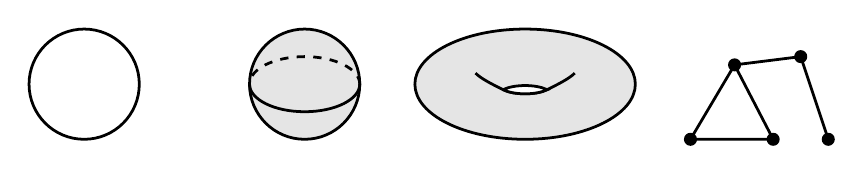
\begin{tikzpicture}[scale=.7]
\newcommand{\vertexradius}{2.5pt}
\newcommand{\vertexscale}{.5}
\newcommand{\bigvertexscale}{1}
\newcommand{\vertex}{\node[circle, fill=black, scale=\vertexscale] }
\newcommand{\highlighta}{red!20}
\newcommand{\highlightb}{blue!20}
\newcommand{\highlightc}{green!20}
\newcommand{\shadinga}{gray!20}
\newcommand{\smallvertex}{\node[circle, fill=black, scale=.2]}
\newcommand{\highlightlinewidth}{3pt}

\tikzset{every path/.style={line width=1 pt}}
    \draw  (-8,1) ellipse (1 and 1);
    \begin{scope}[shift={(2.5,-4)}]
    
    \draw[fill=gray!20]  (-6.5,5) ellipse (1 and 1);
    
    \begin{scope}[]
    \tikzset{every path/.style=};
    \clip  (-8,5) rectangle (-5,4);
    \draw[line width=1pt]  (-6.5,5) ellipse (1 and 0.5);
    \end{scope}
    \begin{scope}[]
    \tikzset{every path/.style=};
    \clip  (-8,6) rectangle (-5,5);
    \draw[dashed, line width=1pt]  (-6.5,5) ellipse (1 and 0.5);
    \end{scope}
    \end{scope}
    \begin{scope}[shift={(2,-4)}]
    \draw[fill=gray!20]  (-2,5) ellipse (2 and 1);
    \draw (-2.9,5.2) .. controls (-2.8,5.1) and (-2.6,5) .. (-2.4,4.9) .. controls (-2.2,4.8) and (-1.8,4.8) .. (-1.6,4.9) .. controls (-1.4,5) and (-1.2,5.1) .. (-1.1,5.2);
    \draw[fill=white] (-2.4,4.9) .. controls (-2.2,5) and (-1.8,5) .. (-1.6,4.9) .. controls (-1.8,4.8) and (-2.2,4.8) .. (-2.4,4.9);
    
    \end{scope}
    
    \begin{scope}[shift={(0.5,0.5)}]
    
    \vertex at (3.3,0.85) {};
    \vertex at (2.5,-0.5) {};
    \vertex at (4,-0.5) {};
    \vertex at (5,-0.5) {};
    \vertex at (4.5,1) {};
    \draw (3.3,0.85) -- (2.5,-0.5) -- (4,-0.5) -- (3.3,0.85) -- (4.5,1) -- (5,-0.5);
    
    \end{scope}\end{tikzpicture}
    \]
Our intuition for continuous maps is that they are the functions between topological spaces which send nearby points to nearby points.
We give a very brief overview of some concepts from topology in \sref{def:topologycc}.

We define the \emph{connected component space of $X$} to be the vector space 
\[C^0(X):=\hom(X, \ZZ_2)\]
of continuous functions from $X$ to the two point set. One can think of this as assigning a color to each connected component of the space $X$, and the number of colorings (determined by the dimension $\dim C^0(X)$) tells you how many connected components there are. 
\[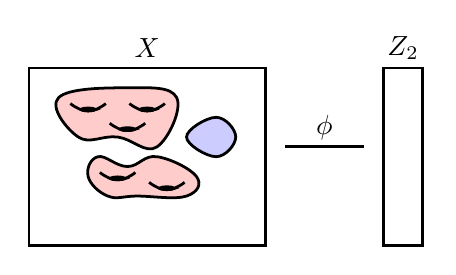
\begin{tikzpicture}[scale=.5]
    \newcommand{\vertexradius}{2.5pt}
\newcommand{\vertexscale}{.5}
\newcommand{\bigvertexscale}{1}
\newcommand{\vertex}{\node[circle, fill=black, scale=\vertexscale] }
\newcommand{\highlighta}{red!20}
\newcommand{\highlightb}{blue!20}
\newcommand{\highlightc}{green!20}
\newcommand{\shadinga}{gray!20}
\newcommand{\smallvertex}{\node[circle, fill=black, scale=.2]}
\newcommand{\highlightlinewidth}{3pt}

\tikzset{every path/.style={line width=1 pt}}
        \begin{scope}[scale=0.5, shift={(-0.5,3)}]
        
        \draw[fill=\highlighta]  plot[smooth cycle, tension=0.7] coordinates {(-4.5,7) (-8,6.5) (-7,4.5) (-5,4.5) (-3,4) (-2,6.5)};
        
        \draw[fill=\highlighta]  plot[smooth cycle, tension=0.7] coordinates {(-6.5,2.5) (-5.5,1.5) (-4,1.5) (-1.5,1.5) (-1,2.5) (-3,3.5) (-4.5,3) (-6,3.5)};
        \draw[fill=\highlightb]  plot[smooth cycle, tension=0.7] coordinates {(-1.5,4.5) (0,3.5) (1,4.5) (0,5.5)};
        
        
        \begin{scope}[shift={(-0.5,-3)}]
        \draw (-2.9,5.2) .. controls (-2.8,5.1) and (-2.6,5) .. (-2.4,4.9) .. controls (-2.2,4.8) and (-1.8,4.8) .. (-1.6,4.9) .. controls (-1.4,5) and (-1.2,5.1) .. (-1.1,5.2);
        \draw[fill=white] (-2.4,4.9) .. controls (-2.2,5) and (-1.8,5) .. (-1.6,4.9) .. controls (-1.8,4.8) and (-2.2,4.8) .. (-2.4,4.9);
        
        \end{scope}
        \begin{scope}[shift={(-3,-2.5)}]
        \draw (-2.9,5.2) .. controls (-2.8,5.1) and (-2.6,5) .. (-2.4,4.9) .. controls (-2.2,4.8) and (-1.8,4.8) .. (-1.6,4.9) .. controls (-1.4,5) and (-1.2,5.1) .. (-1.1,5.2);
        \draw[fill=white] (-2.4,4.9) .. controls (-2.2,5) and (-1.8,5) .. (-1.6,4.9) .. controls (-1.8,4.8) and (-2.2,4.8) .. (-2.4,4.9);
        
        \end{scope}
        \begin{scope}[shift={(-1.5,1)}]
        \draw (-2.9,5.2) .. controls (-2.8,5.1) and (-2.6,5) .. (-2.4,4.9) .. controls (-2.2,4.8) and (-1.8,4.8) .. (-1.6,4.9) .. controls (-1.4,5) and (-1.2,5.1) .. (-1.1,5.2);
        \draw[fill=white] (-2.4,4.9) .. controls (-2.2,5) and (-1.8,5) .. (-1.6,4.9) .. controls (-1.8,4.8) and (-2.2,4.8) .. (-2.4,4.9);
        
        \end{scope}
        \begin{scope}[shift={(-2.5,0)}]
        \draw (-2.9,5.2) .. controls (-2.8,5.1) and (-2.6,5) .. (-2.4,4.9) .. controls (-2.2,4.8) and (-1.8,4.8) .. (-1.6,4.9) .. controls (-1.4,5) and (-1.2,5.1) .. (-1.1,5.2);
        \draw[fill=white] (-2.4,4.9) .. controls (-2.2,5) and (-1.8,5) .. (-1.6,4.9) .. controls (-1.8,4.8) and (-2.2,4.8) .. (-2.4,4.9);
        
        \end{scope}
        \begin{scope}[shift={(-4.5,1)}]
        \draw (-2.9,5.2) .. controls (-2.8,5.1) and (-2.6,5) .. (-2.4,4.9) .. controls (-2.2,4.8) and (-1.8,4.8) .. (-1.6,4.9) .. controls (-1.4,5) and (-1.2,5.1) .. (-1.1,5.2);
        \draw[fill=white] (-2.4,4.9) .. controls (-2.2,5) and (-1.8,5) .. (-1.6,4.9) .. controls (-1.8,4.8) and (-2.2,4.8) .. (-2.4,4.9);
        
        \end{scope}
        \end{scope}
        \vertexa at (4.5,4.5) {};
        \vertexb at (4.5,2) {};
        \draw  (-5,5.5) rectangle (1,1);
        \draw  (4,5.5) rectangle (5,1);
        \draw (1.5,3.5) -- (3.5,3.5);
        \node at (-2,6) {$X$};
        \node at (2.5,4) {$\phi$};
        \node at (4.5,6) {$\mathbb{Z}_2$};
        \end{tikzpicture}\]
    
\begin{claim}[Pullback Map]
    Given a continuous $f: X\to Y$ between topological spaces, there is a map 
    \[f^*: C^0(Y)\to C^0(X).\] 
\end{claim}
\begin{proof}
    The pullback function is defined as before:
    \begin{align*}
        f^*:C^0(Y)\to& C^0(X)\\
        \phi\mapsto& (\phi\circ f)
    \end{align*}
    The only thing to check is that $\phi\circ f$ is a continuous map from $X\to \ZZ_2$; this follows from the composition of continuous maps being continuous. 
\end{proof}
What this claim means is that we can track how the connected components of $X$ are mapped to connected components of $Y$ by using the pullback map.
One interpretation of this is that given a map $f: X\to Y$, we can ``color'' the connected components of $X$ by the connected components of $Y$.

This framework should look very familiar-- it is the same set-up that we used to describe the number of elements in sets.
The connected component space $C^0(X)$ turns questions about connected components into problems in linear algebra instead.
Let us take the annulus, and decompose it into two sets as drawn below. 
This configuration does not respect an inclusion-exclusion like property in the usual sense, in that  $U_1, U_2, X$ each have one connected component, but $U_1\cap U_2$ has two connected components.
\[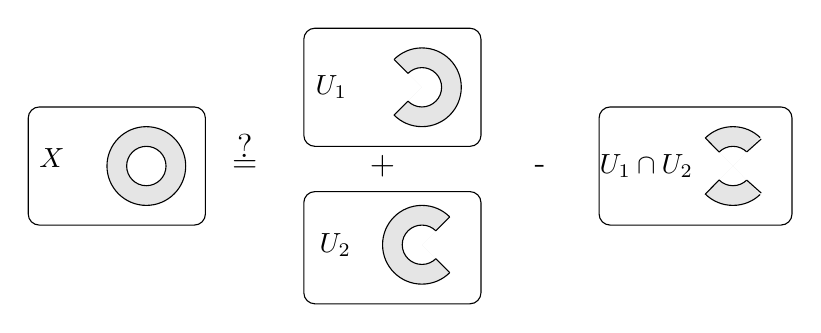
\begin{tikzpicture}[scale=.5]

    \begin{scope}[shift={(-2.5,0)}]
    \draw[rounded corners]  (-5.5,2.5) rectangle (-1,-0.5);
    \draw[fill=gray!20]  (-2.5,1) ellipse (1 and 1);
    \draw[fill=white]  (-2.5,1) ellipse (0.5 and 0.5);
    \node at (-4.9,1.2) {$X$};
    \end{scope}
    
    \begin{scope}[shift={(2,3)}]
    \draw[rounded corners]  (-3,1.5) rectangle (1.5,-1.5);
    \node at (-2.3,0) {$U_1$};\begin{scope}[shift={(2.5,-1)}]
    
    \clip (-2.5,1) -- (-3.65,2.15) -- (-1,2.15) -- (-1,-0.15) -- (-3.65,-0.15) -- cycle;
    \draw[fill=gray!20]  (-2.5,1) ellipse (1 and 1);
    \draw[fill=white]  (-2.5,1) ellipse (0.5 and 0.5);
    \end{scope}
    \draw (135:.5)--(135:1);
    \draw (225:.5)--(225:1);
    \end{scope}
    
    
    \begin{scope}[shift={(9,1)}]
    \draw[rounded corners]  (-2.5,1.5) rectangle (2.4,-1.5);
    \node at (-1.3,0) {$U_1\cap U_2$};\begin{scope}[shift={(3.4,-1)}]
    
    \clip (-2.5,1) -- (-3.65,2.15) -- (-1.4,2.15)-- (-2.5,1) -- (-1.4,-0.15) -- (-3.65,-0.15) -- cycle;
    \draw[fill=gray!20]  (-2.5,1) ellipse (1 and 1);
    \draw[fill=white]  (-2.5,1) ellipse (0.5 and 0.5);
    \end{scope}
    \draw (33:0.6527)--(74:0.7363);
    \draw (-33:0.6527)--(-74:0.7363);
    \draw (16:1.3016)--(23:1.7577);
    \draw (-16:1.3016)--(-23:1.7577);
    \end{scope}
    \begin{scope}[shift={(2,-1)}]
    \draw[rounded corners]  (-3,1.35) rectangle (1.5,-1.5);
    \node at (-2.2,0) {$U_2$};\begin{scope}[shift={(-2.5,-1)}, xscale=-1]
    
    \clip (-2.5,1) -- (-3.65,2.15) -- (-0.5,2) -- (-1,-0.15) -- (-3.65,-0.15) -- cycle;
    \draw[fill=gray!20]  (-2.5,1) ellipse (1 and 1);
    \draw[fill=white]  (-2.5,1) ellipse (0.5 and 0.5);
    \end{scope}
    \draw (45:0.5)--(45:1);
    \draw (-45:0.5)--(-45:1);
    \end{scope}
    \node at (-2.5,1) {\large=};
    \node at (-2.5,1.5) {\large ?};
    \node at (5,1) {\large-};
    \node at (1,1) {\large+};
    \end{tikzpicture}\] 
    
\begin{doubledpage}{example}{Topology 101}{A topological space is a set, equipped with the additional data of \emph{open sets} which determine which points on the topological space are close to each other. In this section, we give a quick overview of point-set topology. }
\label{def:topologycc}
\begin{definition}
    A \emph{topological space} is a pair $(X,\mathcal U)$, where $X$ is a set, and $\mathcal U$ is a specified collection of subsets of $X$, called \emph{open sets} satisfying the following axioms:
    \begin{itemize}
        \item The empty set and whole space $X$ are open sets. 
        \[\emptyset, X\in \mathcal U\]
        \item Any union of open sets is an open set. 
        \[U_\alpha \subset \mathcal U \Rightarrow \left(\bigcup_{\alpha \in A} U_\alpha \right) \in \mathcal U.\]
        \item Any finite intersection of open sets is an open subset. 
        \[\mathcal B\subset \mathcal U , | B|< \infty \Rightarrow \left(\bigcap_{\beta\in B} U_\beta \right) \in \mathcal U.\]
    \end{itemize}
    \end{definition}
    Open sets are kind of strange things. Roughly speaking, if $x$ and $y$ mutually belong to an open set, then we know that they are close to each other in \emph{some} sense, but unlike in the metric space a topology doesn't tell you \emph{how} near two points are two each other. It just tells you that there is something containing both of them. We still get some relative idea of closeness-- if two points mutually belong to many open sets, then we think of them being closer to each other. \\
    Let's introduce a few examples of topologies. 
    \begin{example}[The Discrete Topology]
    Let $X$ be a set. The \emph{discrete topology}  has every subset of $X$ as an open set:
    \[\mathcal U = \{U \;|\; U\subset X\}\]
    This topology has too many open subsets, and all of the points are very far away from each other!
    \end{example}
    A common example of a topological space comes from metric spaces.
    We'll say that a $U$ is open if every point in $x$ is contained within an open ball inside of $U$. 
\newpage
    \begin{example}
    Let $(X, \rho)$ be a metric space. Say that a set $U$ is \emph{$\rho$-open} if for every point $x\in U$, there exists an open ball $B_\epsilon(y)$ with 
    \[x\in B_\epsilon(y)\subseteq U.\]
    Then the collection of sets 
    \[\mathcal U = \{U\subset X \;|\; \text{$U$ is $\rho$-open}\}\]
    makes $(X, \mathcal U)$ a topology. For example, on the real numbers every open interval is an example of an open set with this topology. \label{thm:metrictopology} 
    \end{example}

The interesting maps between topological spaces are those which preserve the topological structure. 
\begin{definition}[Continuous Maps]
    Let $f: X\to Y$ be a function, and $U\subset Y$. The \emph{pre-image} of $Y$ is all the elements of $X$ which get mapped to $U$, 
    \[f^{-1}(U):=\{x\in X\;|\; f(x)\in U\}.\]
    A function $f: X\to Y$ is continuous if and only if for every open set $U\subset Y$, the preimage 
    \[f^{-1}(U)\subset X\]
    is an open set of $X$. 
    \end{definition}
    Suppose that $f: X\to Y$ and $g: Y\to Z$ are continuous maps. Then for any $U\in Z$, $(g\circ f)^{-1}(U)$ is again an open set, which shows that the composition of continuous maps is continuous. 

    A topological space is called \emph{disconnected} if $X=U_1\sqcup U_2$, with $U_1, U_2$ nonempty open sets. The \emph{connected components} of a topological space are the smallest nonempty open sets $\{U_i\}$ so that $X=\bigsqcup_{i=1}^k U_i$. We say that in this case that $X$ has $k$-connected components. 
    \begin{theorem}
        Suppose that $X$ has $k$-connected components. Let $\hom(X, \ZZ_2)$ denote the set of linear maps from $X$ to the space with two points. Then
        \[\dim(\hom(X, \ZZ_2))=k.\] 
    \end{theorem}
\end{doubledpage}
Let's see exactly how the argument from that worked in the proof that $|X|-(|U_1|+|U_2|)+(|U_1\cap U_2|)=0$ fails when we now try to understand the number of connected components. 
The spaces $U_1, U_2, X$ all have one connected component, so 
\[C^0(X)=C^0(U_1)=C^0(U_2)=\ZZ_2.\]
On the other hand, $U_1\cap U_2$ has two connected components, so $C^0(U_1\cap U_2)=\ZZ_2\oplus \ZZ_2$. 
We now look at the inclusions of topological spaces
\[
    \begin{tikzcd}
        U_1\cap U_2 \arrow{r}{i_1} \arrow{d}{i_2} & U_1\arrow{d}{j_1} \\
        U_2\arrow{r}{j_2} & X
          \end{tikzcd}\;\;\;\;\;\;\;
      \begin{tikzcd}
           C^0(U_1\cap U_2 ) &   C^0(U_1) \arrow{l}{i_1^*}\\
           C^0(U_2) \arrow{u}{i_2^*} &  C^0(X) \arrow{u}{j_1^*} \arrow{l}{j_2^*}
      \end{tikzcd}\;\;\;\;\;\;\;
      \begin{tikzcd}
        \ZZ_2\oplus \ZZ_2 &  \ZZ_2 \arrow{l}{i_1^*}\\
        \ZZ_2 \arrow{u}{i_2^*} & \ZZ_2 \arrow{u}{j_1^*} \arrow{l}{j_2^*}
    \end{tikzcd}.
\]
We then condense this down into a sequence of vector spaces by defining $C^1(X):=C^0(U_1)\oplus C^0(U_2)$, and $C^2(X):= C^0(U_1\cap U_2)$. Similarly, we define the maps 
\begin{align*}
    j^*:=j^*_1\oplus j^*_2: C^0(X)\to C^1(X)\\
    i^*:=i^*_1\oplus i^*_2: C^1(X)\to C^2(X).
\end{align*}
as before to give us a sequence of vector spaces and maps between them. 
\[C^0(X)\xrightarrow{j^*}C^1(X)\xrightarrow{i^*}C^2(X)\]
This entire set-up so far follows the same steps as the inclusion-exclusion set up for sets. 
At this point, we deviate from that example. 
\begin{claim}
    For the maps and sets above, the map $j^*$ is injective and  $\im(j^*)\subset \ker(i^*)$.
\end{claim}
\begin{proof}
    Let $\phi:X\to \ZZ_2$ be any continuous function. Then $j^*(\phi)$ is $(j_1)^*\phi\oplus (j_2)^*\phi$, where $(j_1)^*\phi: U_1\to \ZZ_2$ and $(j_2)^*\phi:U_2\to\ZZ_2$ are the restriction of $\phi$ to the subsets $U_1, U_2$. 
    Then 
    \begin{align*}
        (i^*\circ j^*)\phi=(i^*_1\circ j^*_1)\phi+(i^*_2\circ j^*_2)\phi\\
        \intertext{Since $i^*_1j^*_1=i^*_2j^*_2$,}
        =2(i^*_1\circ j^*_1)\phi=0.
    \end{align*}
    This proves that $i^*\circ j^*=0$, which is equivalent to $\im(j^*)\subset \ker(i^*)$. 
\end{proof}
This claim is weaker than the statement that we had for the complex involving sizes of sets. That claim stated that $\im(j^*)=\ker(j^*)$, instead of only having an inclusion, and that $i^*$ was a surjection. 
The discrepancy between these two statements -- equality of image and kernel versus inclusion of image into kernel -- gives us an exact measurement of how the inclusion exclusion principle fails. 
\begin{elevator}[Chain Complexes, Homology, and Chain Maps]
Homological Algebra is a algebraic tool that we'll return to at several points throughout the course, and it makes sense to combine the general facts of the theory in one place. 
\end{elevator}
\begin{definition}[Cochain complexes]  A \emph{cochain complex} is a sequence of vector spaces, $\ldots C^{-1},C^{0},C^{1}\ldots$ and boundary maps $d^n:C^{n}\to C^{n+1}$ with the condition that 
	\[
		d^{n+1}\circ d^{n}=0.
	\] Frequently, we represent a chain complex with the following diagram of vector spaces and maps: 
	\[
\begin{tikzcd}
    \cdots&    C^{1}\arrow{l}{d^{1}} &C^{0} \arrow{l}{d^0}  &C^{-1}\arrow{l}{d^{-1}}& \cdots \arrow{l}{d^{-2}} 
\end{tikzcd}
\]
 We will usually denote the chain complex as $( C^\bullet, d^\bullet)$, where $C^\bullet$ is the sequence of modules and $d^\bullet$ the sequence of boundary maps.
 \footnote{There is no particular reason for the numbers to increase. We could make the numbers decrease, and we would call it \emph{homology} instead.} \label{def:chaincomplex}
\end{definition}
\nomenclature{$(C, d)$}{A chain complex}
\begin{projectdescription}{Abelian Categories}
In principle, all of the tools that we are developing with cochain complexes can be defined with rings and modules instead of just vector spaces. In fact, the field of homological algebra generally works \label{proj:abelian} over any  \emph{Abelian category,} which is a category equipped with the necessary structures to make linear algebra-like constructions. 
\end{projectdescription}
\begin{example}
Let's look at a first example of a chain complex. Let $C^1=C^2= C^3=\RR^2$, so that we may represent our boundary maps by matrices. Consider the sequence of maps 
\[
\begin{tikzcd}[ampersand replacement=\&, column sep= large] 
0 \arrow{r}{0} \& \RR^2 \arrow{r}{\begin{pmatrix}1&0\\0&0\end{pmatrix}} \& \RR^2 \arrow{r}{\begin{pmatrix}0&0\\0&1\end{pmatrix}} \& \RR^2 \arrow{r}{0} \& 0 
\end{tikzcd}
\]
This is an example of a chain complex, as the composition of the differential is zero:
\[d^3\circ d^2 = \begin{pmatrix}0&0\\0&1\end{pmatrix}\cdot \begin{pmatrix}1&0\\0&0\end{pmatrix}=\begin{pmatrix} 0&0\\0&0\end{pmatrix}.\]
\end{example}
The boundary squaring to zero is equivalent to the statement that the image of the boundary map $d^{k}$ is in the kernel of the map $d^{k+1}$.

The theory of cohomology was developed and inspired from techniques in topology, but it is a very useful algebraic framework to have in mind. 
Abstractly, the chain complexes and cohomology are a tool that explains the relations, and relations of relations, and higher meta-relations.
For example, let $V$ be a set with a relation $E\subset V\times V$ on it. Let $\mathcal F(V)$ and $\mathcal F(E)$ be the vector spaces given by maps to the field of two elements.
One might state the relationship now in terms of a map $d: \mathcal F(V)\to \mathcal F(E)$, where the image of a function $\phi:V\to \ZZ_2$ consists of all relations $E$ which have a member evaluating under $\phi$. 

However, the framework of homology allows us to put relations on the set of relations, by introducing maps` $\mathcal F(E)\to \mathcal F(V)$, and so on. 
\begin{example}`'
The example we considered in \sref{hom:thm:inex} is more than just a cochain complex; it satisfies the stronger condition of being \emph{exact} in that $\im d^k=\ker d^{k+1}.$ We'll explore exact complexes in more detail in the future. 
\end{example}
\begin{example}
	The examples considered in \sref{hom:sec:connectedcomplex} of topological spaces covered with sets, and the $\mathcal F(-)$ functor give another example of cochain complexes.
\end{example}
Before we study the general theory of cochain complexes, we would like to build a combinatorial framework for describing topological spaces, which will give us something concrete to stand on when we start describing cochain complexes in this class. 
The natural extension of vertices, edges and faces are building blocks called \textbf{simplices.}
\begin{definition}[Geometric Simplex]
	For $k\geq 0$,  a \textbf{geometric $k$-simplex} $\alpha^k$ is the set of points in $\RR^{k+1}$ whose coordinates are non-negative and sum to $1$. 
	\[\{(x_1, x_2, \ldots,  x_{k+1})\;| \; x_1+x_2+\cdots x_{k+1}=1,  x_i\geq 0\}.\]
	Given a simplex,  we say that $k$ is the \textbf{dimension} of $\alpha^k$. 
\end{definition}

\begin{example}
	We've already seen a couple of geometric simplices before, and given them some common names.\\
\begin{tabular}{l|l|b{5cm}|c}
Dim &  Name & Notes & Graphical Representation\\ \hline
	0 & Vertex &  By the above definition,  it specifically the point $1\in \RR^1$.  & \begin{tikzpicture}[scale=.7]
\draw[->,  dotted] (-2, 0)--(2, 0);
\fill(1,0) circle[radius=.1];
\end{tikzpicture}\\\hline
1 & Edge & Drawn with the above notation, it is the line segment in the first quadrant. Notice that the restriction of the line to either axis gives us a point.  &
			\begin{tikzpicture}[scale=.5]
				\draw[->,  dotted] (-2, 0)--(2, 0); \draw[->,  dotted] (0, -2)--(0, 2);
				\draw (1, 0)--(0, 1);
			\end{tikzpicture}\\\hline
0 & Face & A 2-simplex is a (filled in) triangle, filling the first quadrant. Again, the restriction to either the coordinate planes or axis gives us edges and vertices respectively. & 			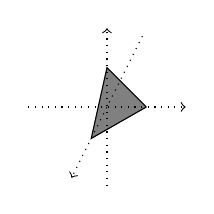
\begin{tikzpicture}[scale=.5]
				\draw[fill=gray] (1, 0)--(0, 1)--(-.4,  -.8)--(1, 0);
				\draw[->,  dotted] (-2, 0)--(2, 0); \draw[->,  dotted] (0, -2)--(0, 2) ; \draw[->,  dotted] (.9,  1.8)--(-.9,  -1.8) ;
			\end{tikzpicture}
\end{tabular}
\end{example}
Simplices have the property that their boundaries are created of smaller simplices. For instance,  a 2-simplex (triangle) has 3 boundary 1-simplices (edges.) A 3-simplex (tetrahedron) has 4 boundary 1-simplices. In general a $k$-simplex has $k+1$ boundary $k-1$-simplices,  called \emph{facets}.

A simplex has more than just $k-1$ dimensional facets; it also has boundary components of dimension $k-l$. Each boundary component is uniquely specified by the $k-l+1$ corner vertices it uses. If we wanted to build more complicated spaces by gluing together simplices, one would imagine that we would take these simplices and join them together along boundary strata picked out by identifying their vertices.

\begin{examplefigureenv}[A simplicial complex]{191figures/simp_examplecomplex.tikz}
	Here is an example of a topological space constructed from simplices. It uses 8 vertices, has 13 edges, 8 faces, and 1 3-simplex (the right simplex is not filled in.) Notice that this topological space doesn't have a consistent notion of ``dimension''-- the dimension varies from 1-3 dimensional depending on which part of the complex you look at.
\end{examplefigureenv}

In practice, it is simpler to build in this identification of simplices from the very beginning.   
\begin{definition}[Abstract Simplicial Complex]
	A \emph{finite abstract simplicial complex} is a pair $X=(\Delta, \mathcal S)$ where
	\begin{itemize}
	\item  $\mathcal S$ is a base set of vertices
	\item $\Delta\subset \mathcal P(S)$ is a finite set of \emph{simplices} 
	\end{itemize}
	where the simplices are downward closed. This means that whenever $\sigma\in \Delta$ and $\tau\subset \sigma$, then $\tau\in \Delta$. We say that $\sigma\in \Delta$ is a \emph{$k$-simplex} if $|\sigma|=k+1.$ We will in this case write that $\dim(\sigma)=k$. 
	If $\sigma\subset \tau$, and $\dim\sigma=\dim\tau-1$, then we say that $\sigma$ is a \emph{facet} of $\tau$ and write $\sigma \lessdot \tau$. 
	
\end{definition}

%\begin{example}[Graph Complex]
%A simple example of a cochain complex comes from our exploration of graph theory.
%Let $V$ and $E$ be the edges and vertices of a graph. There exist left and right boundary maps %$\partial_l:E\to V$ and $\partial_r: E\to V$ sending each edge to its left or right boundary.
%We define 
%\begin{align*}
%	d: \mathcal F(V)\to& \mathcal F(E)\\
%	\phi\mapsto& (\partial_l\oplus\partial_r)^*\phi
%\end{align*}
%to be the differential map. 
%Note that $d(\phi)=0$ and the graph $G$ is connected, then for all $v$ either $\phi(v)=0$ or %$\phi(v)=1$.
%\end{example}
%\begin{example}[Embedded Graph Complex]
%Recall, if we have a net $G$ for a surface $\Sigma$, we get an associated chain complex in %Definition \ref{def:surfacecomplex}. This chain complex can be modified to capture the full %topological data of $\Sigma$. In a way similar to the graph complex, vertices are related if %there exists a path between them. However, in this example, we have a higher relation: paths are %related if there exists a subsurface which has that path as it's boundary. 
%\end{example}
%\begin{example}[Simplicial Homology]
%The Chain complex associated to a simplicial complex \ref{def:simplicialhomology} is the natural %generalization of the previous two constructions. The elements of this chain complex are %$k$-dimensional sub-complexes, and two subcomplexes are related if they are the boundary %components of a common $k+1$ dimensional subcomplex.
%\end{example}
%While the examples that we've looked at in class are inspired from topology, there are many examples come from different branches of mathematics. 
\begin{claimfigureenv}[Covers from Simplices]{191figures/simp_examplecovering.tikz}
	Let $X=(\Delta, \mathcal S)$. There is a collection of sets $\{U_s\}_{s\in \mathcal S}$ so that $\bigcup_{s\in \mathcal S} U_s=X$.
	Define for each simplex $\sigma\in \Delta$ the associated covering set 
	\[U_{I}=X\cap \bigcap_{s\in I}U_s.\]
	Furthermore, for every indexing set $I$,  $U_I$ is contractible, and is non-empty if and only if $I=\sigma$ for some simplex in our complex. 

	Note that for each $\sigma\lessdot\tau$, there exists an inclusion map $i_{\sigma\tau}:U_\tau\to U_\sigma$, and subsequently a map 
	\[i^*_{\sigma\tau}: \hom(U_\sigma, \ZZ_2)\to \hom(U_\tau, \ZZ_2).\]
\end{claimfigureenv}
We now define the \emph{reduced Cech cochain complex.} For each $i$, let
\[\underline C^{-1}(X, \ZZ_2):= \hom(X, \ZZ_2)\]
\[\underline C^i(X, \ZZ_2):= \bigoplus_{\sigma\;|\; \dim(\sigma)=i} \hom(U_\sigma, \ZZ_2).\]
Define the differential maps 
\begin{align*}
	d^i&: \underline C^i(X, \ZZ_2)\to C^{i+1}(X, \ZZ_2)\\
	d^i&:=\bigoplus_{\sigma\lessdot\tau, \dim\sigma=i} i^*_{\sigma\tau}.
\end{align*}
\begin{claim}[Simplicial Cochains are a complex]
	$\underline C^\bullet(X, \ZZ_2)$ with differential $d^i$ is a cochain complex. Furthermore, a basis of the $C^i$ can be indexed by the $i$-dimensional simplices of $X$, and the differential defined on a basis element $e_\sigma$ can be written as 
	\[
		d(e_\sigma)=\sum_{\tau\;|\; \sigma\lessdot \tau} e_\tau.
	\]
\end{claim}
It is rarely the case that this will be an example of an exact chain complex. The difference between $\im d^{i+1}$ and $\ker d^i$ will be an interesting thing to measure.
Because we are loathsome to leave the land of vector spaces, we will measure this difference with a new vector space. 

\begin{definition}[Cohomology Groups]
	Let $(C,\partial_\bullet)$ be a chain complex.
	The \emph{cohomology} of $C^\bullet$ at $n$ is defined to be the module 
\[H^n(C)=\frac{\ker d^{n}}{ \im d^{n-1}}\]
 As the composition $d^{n+1}\circ d^n=0$, this is well defined.
 \label{def:homologygroups}
\end{definition}
\nomenclature{$H^k(C)$}{The $k$-th homology group of $(C, \partial)$}
For convenience, we will often call the kernel of $d^{n}$ the set of cocycles, and write it $Z^n$. The image of $d^{n-1}$ is the set of coboundaries and will be written $B^n$. Then $H^n(C)=Z^n/B^n$. The names cycles and boundaries correspond to the geometric interpretation of the homology as given above.  
\begin{definition} 
	We say that a chain complex is \emph{bounded} if there exists $n$ such that $C^i=0$ if $|i|\geq n$.
\end{definition}
While it doesn't make sense to ask about the dimension of a chain complex, there is a generalization of dimension which applies to chain complexes. 
\begin{definition}[$\chi$ of a complex]
Let $(C, d)$ be a bounded cochain complex  with each $C^i$ of finite dimension.
 Then the \emph{Euler Characteristic} of $(C, d)$ is the integer 
\[\chi(C, d):= \sum_{k=-\infty}^\infty (-1)^k \dim (C^k).\]
\end{definition}
Notice that the Euler Characteristic has no dependence on the differential of a chain complex. However, it is intimately related to the chain structure through an application of the rank-nullity theorem.  
\nomenclature{$\chi(C, d)$}{The Euler Characteristic of a Chain Complex}
\begin{lemma}[Euler via Homology] Suppose that the chain complex is bounded. Then 
	\[\chi(C, d) =\sum_{k=-\infty}^\infty (-1)^k \dim H^k.\]
\label{lemma:eulercharacteristic}
\end{lemma}
\begin{proof} Because our complex is bounded, there exists $n$ such that $|k|\geq n$ implies that $C^k=H^k=0$.
	Then we proceed by computing the sum:
\begin{align*}
\chi(C, d)=&\sum_{k=-i}^{i}(-1)^k C^k\\
\intertext{Applying the Rank-Nullity theorem}
 &=\sum_{k=-i}^{i}(-1)^k (\dim (\ker d^k )+\dim( \im d^k))\\
 \intertext{Shifting the sum}
 &=\sum_{k=-i}^{i}(-1)^k (\dim(\ker d^k)-\sum_{k=-i}^{i}(-1)^{k-1} \dim( \im d^k))\\
 &=\sum_{k=-i}^{i}(-1)^k \dim( \ker d^k) - \dim (\im d^{k-1})\\&= \sum_{k=-i}^{i}(-1)^k \dim H^k\end{align*}
\end{proof}

One interpretation of homology is that it is an algebraic measure of how far a sequence strays from being \emph{exact.} \label{append:chaincones}
\begin{definition}[Exact Sequences]
A chain complex $(C, d)$ is called \emph{exact} if $H^k(C)=0$ for all $k$. \label{def:exactsequence} 
\end{definition}
Notice by \sref{lemma:eulercharacteristic}, whenever $(C, d)$ is exact, the Euler characteristic  $\chi(C, d)=0$. 
\begin{corollary}
	Inclusion-Exclusion holds for sets. 
\end{corollary}
\begin{proof}
	In \sref{hom:thm:inex} we showed that the chain complex dictating inclusion-exclusion for sets was exact. Furthermore, we showed that the inclusion-exclusion principle for sets was equivalent to $\chi(A, d)=0$. 
\end{proof}
\begin{elevator}[Maps between chain complexes, addition and subtraction]
	
\end{elevator}
Now that we have chain complexes, we want to look at functions that can go between them. Just like when we study vector spaces and groups, it is only useful to study the maps between these objects which preserve their structure. We want the function between chain complexes to be compatible with the differential.
\begin{definition}[Chain map] \label{def:chainmap} 
	Let $( A,d_A)$ and $( B, d_B)$ be chain complexes, and let $f^i:A^i\to B^i$ be a collection of maps. Then we say that $f^\bullet=\{f^i\}$ is a \emph{cochain map} if the following diagram commutes for all $i$:
\[\begin{tikzcd}
	A^i\arrow{r}{d^i_A}\arrow{d}{f^i}&A^{i+1}\arrow{d}{f^{i+1}}\\ B^i\arrow{r}{d^i_B} &B^{i+1} 
\end{tikzcd}.\] 
\end{definition} 
A chain map not only preserves the boundary structure of the chain complex, it also gives us maps between their homology groups. 
\begin{claim}[Induced map on cohomology]
Let $f^\bullet:(A, d_A)\to (B, d_B)$ be a chain map. Then there is a well defined map between the cohomology of $(A, d_A)$ and $(B, d_B)$ given by 
\begin{align*}
f^k: H^k(A)\to& H^k(B)\\
[a]\mapsto& [f^k(a)]. 
\end{align*}
\end{claim}
\begin{proof}
In order to show that this map is well defined, we need to check two things.  First we must show  that elements representing homology classes in $A$ get sent to elements representing homology classes in $B$.
Second, we must show that resulting map does not depend on the choice of representative for $a$. 
\begin{itemize}
\item For the first part, let $[a]\in H^k(A)$ be an element of homology. In order for $[f^k(a)]$ to be an element of $H^k(B)$, we need that $f^k(a)\in \ker d_B.$ We make a computation:
\begin{align*}
d_B(f^k(a))=& f^{k+1}(d_A(a))
\intertext{Since $[a]\in H^k(A)$, we know that $a\in \ker d_A$. }
=& f^{k+1}(0)=0. 
\end{align*}
\item For the second part, suppose we have 2 different representatives of the same cohomology class $[a]=[a']\in H^k(A)$. We would like to show that $[f^k(a)]=[f^k(a')]\in H^k(B)$. \\
Two classes in homology are equivalent if they differ by an element in the image of $d^{k-1}$. Therefore, we can prove the statement by finding an element $\beta\in B^{k-1}$ which satisfies:
\[[f^k(a)]-[f^k(a')]=d^{k-1}(\beta).\]
We can construct this $\beta$ by looking at the difference $a-a'.$  Since $[a]=[a']$, there is an element $\alpha\in C^{k-1}(A)$ so that $d_A(\alpha)=a-a'$. \\
We now are in the place to make a computation. 
\begin{align*}
f^k(a)-f^k(a')=& f^k(a-a')\\
=& f^k(d_A(\alpha))\\
=& d_B(f^{k-1}(\alpha)).
\end{align*}
We set $\beta=f^{k-1}(\alpha)$ to realize the equivalence relation between the two homology classes $[f^k(a)], [f^k(a')]$. 
\end{itemize}
\end{proof}
The most useful example of exact complexes are \emph{short exact sequences}, which are exact complexes of the form:
\[\begin{tikzcd} 0 \arrow{r} & A \arrow{r}{i} & B \arrow{r}{\pi} & C \arrow{r} & 0 \end{tikzcd}.\]
From the definition of exactness $i: A\to B$ must be injective, and $\pi: B\to C$ must be surjective. 
If we were only interested in vector spaces, then $B=A\oplus C$ would be the only interesting data about this exact complex.
If we think of $A, B,$ and $C$ as being the generalizations of the numbers $\dim(A), \dim(B)$ and $\dim(C)$, then a short exact sequence is a way to encode that $\dim(A)+\dim(C)=\dim(B)$. 

In the world of chain complexes, $B$ could contain more data than just that of the vector spaces $A\oplus C$ -- we need to additionally consider the information that comes from a differential.
\begin{definition}
Let $(A, d_A), (B, d_B), (C, d_C)$ be chain complexes. Let $i^\bullet: A^\bullet\to B^\bullet$ and $\pi^\bullet: B^\bullet\to C^\bullet$ be maps of cochain complexes. We say that 
\[\begin{tikzcd} 0 \arrow{r} & A^\bullet \arrow{r}{i^\bullet} & B^\bullet \arrow{r}{\pi^\bullet} & C_\bullet \arrow{r} & 0 \end{tikzcd}\] 
is a short exact sequence of chain complexes if for all $k$, 
\[\begin{tikzcd} 0 \arrow{r} & A^k \arrow{r}{i^k} & B^k \arrow{r}{\pi^k} & C^k \arrow{r} & 0 \end{tikzcd}\] 
is a short exact sequence of vector spaces. 
\end{definition}
The theory of short exact sequences of chain complexes is a lot richer than the theory for vector spaces, because chain complexes contain much more internal structure. 
We will now associate to each map $f^\bullet: A^\bullet\to B^\bullet$ a canonical short exact sequence.   
\begin{definition}[Cone of Chain morphism]
Let $f^\bullet:A^\bullet\to B^\bullet$ be a map of cochain complexes. Define the \emph{cone of $f$,} to be the cochain complex with 
\begin{itemize}
\item Chain groups $\cone^{k}(f)=A^{k+1}\oplus B^{k}$
\item Differential defined by $d^k_{\cone}(a, b)= (-d_A^{k+1}(a), d^{k}_B(b)+f^{k+1}(a))$. 
\end{itemize}
\label{def:chaincone}
\end{definition}
Note that for each $k$, $A^{k+1}\to \cone^k(f)\to B^k$ is a short exact sequence.
We should think of $\cone^\bullet(f)$ as being the chain complex created by ``attaching'' $A^{\bullet+1}$ to $B^\bullet$. 
\begin{claim}[Mapping cone is complex]
$\cone^\bullet(f)$ is a cochain complex. 
\end{claim}
\begin{proof}
A convenient notation for this proof will be to think of $d^k_{\cone}$ as having the form of a matrix:
\[
d^k_{\cone}=\begin{pmatrix} -d_A^{k+1}&0\\ f^{k+1} & d^{k}_B \end{pmatrix}.
\]
We can then compute $d^{k+1}_{\cone}\circ d^k_{\cone}$ by using matrix multiplication. 
\begin{align*}
d^{k+1}_{\cone}d^k_{\cone}=&
\begin{pmatrix} 
	-d_A^{k+2}&0\\ 
	f^{k+2} & d^{k+1}_B
 \end{pmatrix}
\begin{pmatrix}
 -d_A^{k+1}&0\\
 f^{k+1} & d^{k}_B 
\end{pmatrix}\\
=&\begin{pmatrix} 
d_A^{k+2}\circ d^{k+1}_A & 0\\
d_B^{k+1}\circ f^{k+1} - f^{k+2}\circ d_A^{k+1} & d^{k+1}_B\circ d^{k}_B
\end{pmatrix}
\intertext{Using the definitions of chain map and chain differential,}
=& \begin{pmatrix} 0&0\\0&0\end{pmatrix}.
\end{align*}
\end{proof}
The cone of a morphism $f^\bullet: A^\bullet\to B^\bullet$ fits into a short exact sequence of chain complexes, 
\[ \begin{tikzcd}
0 \arrow{r} & B^{\bullet} \arrow{r}{i}&\cone^\bullet(f) \arrow{r}{\pi} & A^{\bullet+1}\arrow{r} & 0 
\end{tikzcd}
\]
where $i, \pi $ are the natural inclusion and projection maps. Notice the shift in the index on the left hand side. A piece of notation that we will use for this shift in index is 
\[C^{\bullet-1}=C^\bullet[-1].\] 
\nomenclature{$C_\bullet[1]$}{The chain complex $C_\bullet$ shifted by $1$ in index}
The way that $A^{\bullet+1}$ is glued to $B^\bullet$ is dictated by the map $f^{\bullet}$. 
In this way, the exact sequence of chain complexes not only remembers that we can put $A^{\bullet+1}, B^{\bullet}$ together to build $\cone^{\bullet}$, but 
also \emph{how} these things were glued together. 

From this short exact sequence, we surprisingly get a \emph{long exact sequence} of homology groups. 
\begin{theorem}[SES-LES for mapping cones]
Let $f^\bullet: A^\bullet\to B^\bullet$ be a chain map. 
We have a short exact sequence of chain complexes
\[ \begin{tikzcd}
	0 \arrow{r} & B^{\bullet} \arrow{r}{i}&\cone^\bullet(f) \arrow{r}{\pi} & A^\bullet[1]\arrow{r} & 0 
	\end{tikzcd}
\]
And we have the following long exact sequence of homology groups:
\[
	\begin{tikzcd}
\cdots \arrow{r}{f} & H^k(B)\arrow{r}{i} & H^k(\cone(f)) \arrow{r}{\pi} &  H^k(A[1]) \arrow{r}{f}  & H^{k+1}(B) \arrow{r} & \cdots
\end{tikzcd}.
\]
\label{thm:leqfromcone}
\end{theorem}
\begin{proof}
Showing that this is a long exact sequence amounts to checking that the sequence is exact at $H^k(B), H^k(\cone(f)),H^k(A[1]).$
We will show that the function is exact at $H^k(\cone(f))\to H^k(A[1])\to H^{k+1}(B)$, which is perhaps the most surprising statement in the proof. 
To show the isomorphism 
\[\ker(f: H^k(A[1])\to H_{k+1}(B))\simeq \im( \pi: H^k(\cone(h))\to H^k(A[1]),\]
we will show two inclusions. 

We prove that $\ker(f: H^k(A[1])\to H^{k+1}(B))\subset \im( \pi: H^k(\cone(f))\to H^k(A[1]).$ Take a cohomology class $[a]\in H^k(A[1])$ which is in the kernel of $f$ so that
\[f([a])=[0].\] 
Since $\cone^k(f)=A^k[1]\oplus B^k$, a natural candidate for an element of $\cone^k(f)$ whose image under $\pi$ is $a$ would be $(a, 0)$. 
However, it may not be the case that this a homology class, as 
\[d_{\cone}(a, 0)=( d_A a, f(a))\]
which is not necessarily zero. 
As $[a]\in H^k(A[1])$, we are guaranteed that $d_A a=0$. However, the only data that we have about $f(a)$ is that it is \emph{cohomologous} to $0$. Since $f([a])=[0]$, there is an element $b\in B^k$ realizing the equivalence relation via  $f(a)=d_B b$. Replacing our candidate element\footnote{The notation $\pi^{-1}(a)$ means that we have picked \emph{an} inverse image of $a$ under $\pi$. 
However, the map $\pi$ is usually not invertible, and choices were made to produce this inverse image. In short, $\pi^{-1}$ is not a map.} with 
\[\pi^{-1}(a):= (a, -b)\]
we can compute 
\begin{align*}
\pi (\pi^{-1}(a))= &\pi(a, -b) = a\\
d^{\cone}( \pi^{-1}(a) )=& d_{\cone} (a, -b) = 0
\end{align*}
Therefore, $\ker(f: H^k(A[1])\to H^{k+1}(B))\subset \im( \pi: H^k(\cone(f))\to H^k(A[1]).$

The other direction is that $\ker(f: H^k(A[1])\to H^{k+1}(B))\supset \im( \pi: H^k(\cone(f))\to H^k(A[1]).$ To show this, we need to show that the composition of $f\circ \pi=0$ on cohomology. 
Let $[(a, b)]\in H^k(\cone(f))$ be any element of homology. 
Since this is an element of homology, $d_{\cone}(a, b)=0$, and in particular,
\[f(a)= - d_B b. \]
We can use this when computing:
\begin{align*}
f\circ \pi[(a, b)] =& f[(a)]=[-d_B b ]=[0].
\end{align*}
We omit the arguments for showing exactness at the other portions of the sequence.
\end{proof}
This is sometimes notated in the following way:
\[\begin{tikzcd}
	\cdots     \arrow{r}{i} \arrow[draw=none]{d}[name=Z, shape=coordinate]{}&H^{n  }(\cone(f)) \arrow{r}{\pi} & H^{n  }(A[1]) \arrow[rounded corners,to path={ -- ([xshift=2ex]\tikztostart.east)|- (Z) [near end]\tikztonodes-| ([xshift=-2ex]\tikztotarget.west)-- (\tikztotarget)}]{dll}{f} \\
	H^{n+1}(B) \arrow{r}{i} \arrow[draw=none]{d}[name=Z, shape=coordinate]{}&H^{n+1}(\cone(f)) \arrow{r}{\pi} & H^{n+1}(A[1]) \arrow[rounded corners,to path={ -- ([xshift=2ex]\tikztostart.east)|- (Z) [near end]\tikztonodes-| ([xshift=-2ex]\tikztotarget.west)-- (\tikztotarget)}]{dll}{f} \\
	H^{n+2}(B) \arrow{r}{i} &                                                H^{n+2}(\cone(f)) \arrow{r}{\pi} &\cdots 
\end{tikzcd}
\]
There is a useful corollary that follows from this construction:
\begin{corollary}[2-out of 3]
Suppose that $A^\bullet, B^\bullet$ are exact, and let $f^\bullet: A^\bullet\to B^\bullet$ be any map. Then $\cone^\bullet(f)$ is exact. 
\end{corollary}
\begin{proof}
	By assumption $H^k(A)=H^k(B)=0$ for all $k$. Therefore, we have the long exact sequence
	\[\begin{tikzcd}
		\cdots     \arrow{r}{i} \arrow[draw=none]{d}[name=Z, shape=coordinate]{}&H^{n  }(\cone(f)) \arrow{r}{\pi} & 0 \arrow[rounded corners,to path={ -- ([xshift=2ex]\tikztostart.east)|- (Z) [near end]\tikztonodes-| ([xshift=-2ex]\tikztotarget.west)-- (\tikztotarget)}]{dll}{f} \\
		0          \arrow{r}{i} \arrow[draw=none]{d}[name=Z, shape=coordinate]{}&H^{n+1}(\cone(f)) \arrow{r}{\pi} & 0 \arrow[rounded corners,to path={ -- ([xshift=2ex]\tikztostart.east)|- (Z) [near end]\tikztonodes-| ([xshift=-2ex]\tikztotarget.west)-- (\tikztotarget)}]{dll}{f} \\
		0          \arrow{r}{i} &                                                H^{n+2}(\cone(f)) \arrow{r}{\pi} &\cdots 
	\end{tikzcd}
	\]
	from which it follows that $H^k(\cone(f))=0$ for all $k$. Therefore $\cone^\bullet(f)$ is exact. 
\end{proof}

\begin{doubledpage}{theorem}{Inclusion-Exclusion}{
	Let $X$ be a set with a decomposition into smaller subsets, $X=\bigcup_{i\in I} U_i$. Let $U_J=\cap_{j\in J} U_i$. There exists an exact chain complex $CR^\bullet(\mathcal U)$ with $CR^\bullet(\mathcal U)=\bigoplus_{J\subset I, |J|=k} \mathcal F(U_J)$. }
	
\[
	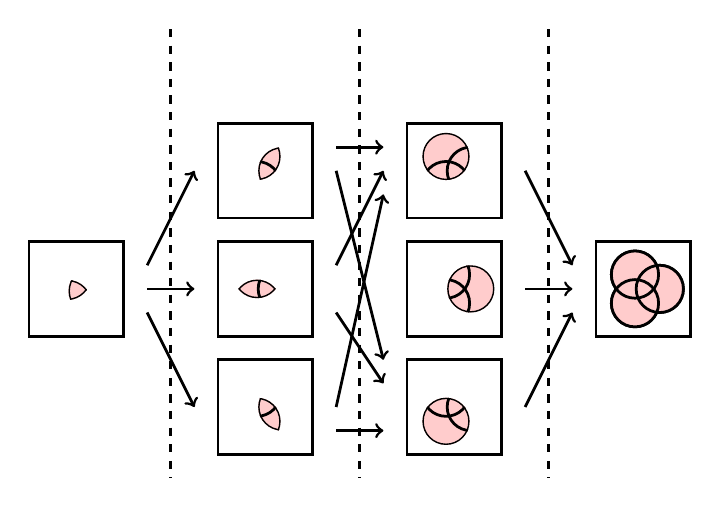
\begin{tikzpicture}[scale=.3]

\begin{scope}[shift={(-24,2)}]
\draw[line width = 1pt]  (13,-3) rectangle (17,-7);
\clip (-17:15.2947) circle[radius=1];
\clip (-18:16.477) circle[radius=1];
\clip (-21:15.6861) circle[radius=1];
\fill[red!20] (-17:15.2947) circle[radius=1];
\fill[red!20] (-18:16.477) circle[radius=1];
\fill[red!20] (-21:15.6861) circle[radius=1];
\draw[line width = 1pt] (-17:15.2947) circle[radius=1];
\draw[line width = 1pt] (-18:16.477) circle[radius=1];
\draw[line width = 1pt] (-21:15.6861) circle[radius=1];
\end{scope}\begin{scope}[shift={(15,-3)}]
\draw[line width = 1pt]  (-2,2) rectangle (2,-2);
\draw[line width = 1pt] (120:0.7) circle[radius=1];
\draw[line width = 1pt] (0:0.7) circle[radius=1];
\draw[line width = 1pt] (240:0.7) circle[radius=1];
\fill[red!20] (120:0.7) circle[radius=1];
\fill[red!20] (0:0.7) circle[radius=1];
\fill[red!20] (240:0.7) circle[radius=1];
\draw[line width = 1pt] (120:0.7) circle[radius=1];
\draw[line width = 1pt] (0:0.7) circle[radius=1];
\draw[line width = 1pt] (240:0.7) circle[radius=1];
\end{scope}\begin{scope}[shift={(7,2)}]
\draw[line width = 1pt]  (-2,2) rectangle (2,-2);
\clip (120:0.7) circle[radius=1];
\draw[line width = 1pt] (0:0.7) circle[radius=1];
\draw[line width = 1pt] (240:0.7) circle[radius=1];
\fill[red!20] (120:0.7) circle[radius=1];
\fill[red!20] (0:0.7) circle[radius=1];
\fill[red!20] (240:0.7) circle[radius=1];
\draw[line width = 1pt] (120:0.7) circle[radius=1];
\draw[line width = 1pt] (0:0.7) circle[radius=1];
\draw[line width = 1pt] (240:0.7) circle[radius=1];
\end{scope}\begin{scope}[shift={(7,-3)}]
\draw[line width = 1pt]  (-2,2) rectangle (2,-2);
\clip (0:0.7) circle[radius=1];
\draw[line width = 1pt] (120:0.7) circle[radius=1];
\draw[line width = 1pt] (240:0.7) circle[radius=1];
\fill[red!20] (120:0.7) circle[radius=1];
\fill[red!20] (0:0.7) circle[radius=1];
\fill[red!20] (240:0.7) circle[radius=1];
\draw[line width = 1pt] (120:0.7) circle[radius=1];
\draw[line width = 1pt] (0:0.7) circle[radius=1];
\draw[line width = 1pt] (240:0.7) circle[radius=1];
\end{scope}\begin{scope}[shift={(7,-8)}]
\draw[line width = 1pt]  (-2,2) rectangle (2,-2);
\clip (240:0.7) circle[radius=1];
\draw[line width = 1pt] (120:0.7) circle[radius=1];
\draw[line width = 1pt] (0:0.7) circle[radius=1];
\fill[red!20] (120:0.7) circle[radius=1];
\fill[red!20] (0:0.7) circle[radius=1];
\fill[red!20] (240:0.7) circle[radius=1];
\draw[line width = 1pt] (120:0.7) circle[radius=1];
\draw[line width = 1pt] (0:0.7) circle[radius=1];
\draw[line width = 1pt] (240:0.7) circle[radius=1];
\end{scope}\begin{scope}[shift={(-1,2)}]
\draw[line width = 1pt]  (-2,2) rectangle (2,-2);
\clip (120:0.7) circle[radius=1];
\clip (0:0.7) circle[radius=1];
\draw[line width = 1pt] (240:0.7) circle[radius=1];
\fill[red!20] (120:0.7) circle[radius=1];
\fill[red!20] (0:0.7) circle[radius=1];
\fill[red!20] (240:0.7) circle[radius=1];
\draw[line width = 1pt] (120:0.7) circle[radius=1];
\draw[line width = 1pt] (0:0.7) circle[radius=1];
\draw[line width = 1pt] (240:0.7) circle[radius=1];
\end{scope}\begin{scope}[shift={(-1,-3)}]
\draw[line width = 1pt]  (-2,2) rectangle (2,-2);
\clip (120:0.7) circle[radius=1];
\clip (240:0.7) circle[radius=1];
\draw[line width = 1pt] (0:0.7) circle[radius=1];
\fill[red!20] (120:0.7) circle[radius=1];
\fill[red!20] (0:0.7) circle[radius=1];
\fill[red!20] (240:0.7) circle[radius=1];
\draw[line width = 1pt] (120:0.7) circle[radius=1];
\draw[line width = 1pt] (0:0.7) circle[radius=1];
\draw[line width = 1pt] (240:0.7) circle[radius=1];
\end{scope}\begin{scope}[shift={(-1,-8)}]
\draw[line width = 1pt]  (-2,2) rectangle (2,-2);
\clip (0:0.7) circle[radius=1];
\clip (240:0.7) circle[radius=1];
\draw[line width = 1pt] (120:0.7) circle[radius=1];
\fill[red!20] (120:0.7) circle[radius=1];
\fill[red!20] (0:0.7) circle[radius=1];
\fill[red!20] (240:0.7) circle[radius=1];
\draw[line width = 1pt] (120:0.7) circle[radius=1];
\draw[line width = 1pt] (0:0.7) circle[radius=1];
\draw[line width = 1pt] (240:0.7) circle[radius=1];
\end{scope}




\draw[line width = 1pt][dashed] (-5,8) -- (-5,-11);
\draw[line width = 1pt][dashed] (3,8) -- (3,-11);
\draw[line width = 1pt][dashed] (11,8) -- (11,-11);
\draw[line width = 1pt,->] (-6,-2) -- (-4,2);
\draw[line width = 1pt,->] (-6,-3) -- (-4,-3);\draw[line width = 1pt,->] (-6,-4) -- (-4,-8) ;\draw[line width = 1pt,->](2,3) -- (4,3);\draw[line width = 1pt,->] (2,2) -- (4,-6) ;\draw[line width = 1pt,->](2,-9) -- (4,-9) ;\draw[line width = 1pt,->](2,-8) -- (4,1);\draw[line width = 1pt,->] (2,-4) -- (4,-7) ;\draw[line width = 1pt,->](2,-2) -- (4,2) ;\draw[line width = 1pt,->](10,-8) -- (12,-4);\draw[line width = 1pt,->] (10,-3) -- (12,-3) ;\draw[line width = 1pt,->](10,2) -- (12,-2);
\end{tikzpicture}
\]
We will prove this theorem by using the tools of homological algebra, and induct on the size of $I$. 
\begin{definition}
	Let $\mathcal U=\{U_i\}_{i\in I}$ be a collection of subsets which cover $X$. Denote by 
	$\mathcal U_{\cap}:= \{U_j\}_{}$
\end{definition}

A covering $\mathcal U=\{U_i\}$ of $X$  is a collection of subsets $U_i\subset X$ so that  \[X=\bigcup_{i\in I} U_i.\]
To each covering of $X$ we will create an \emph{resolution complex} $CR_\bullet(\mathcal U)$.
\begin{definition}
Let $\mathcal U=\{U_i\}_{i\in I}$ be a covering of $X$. For each $J\subset I$, define the subset $U_J:=X\cap (\bigcap_{i\in J} U_i)$.
Suppose that $J$ and $K$ differ by a single index. We will then write $J\lessdot K$. Notice that whenever $K\gtrdot J$ we have an inclusion map $i_{K\gtrdot J}:U_K\to U_J$, and therefore we get an associated map 
\[i_{K\gtrdot J}^*: \mathcal F (U_J)\to \mathcal F(U_K).\]
We define the chain groups 
\[CR^k(\mathcal U):=\bigoplus_{K\subset I, |K|=k} \mathcal F(U_K)\]
and define the differential map to be
\[d^k_{CR}:=\bigoplus_{K\gtrdot J} i_{K\gtrdot J}^*.\]
\end{definition}
We will show that this gives us a chain complex by constructing it in a different fashion. 

\begin{lemma}
	Let $\hat U_1$ be the elements of $X$ which only belong to $U_1$,   Let $\mathcal U_X=\{U_i\}_{i\in I}$ be a cover of $X$. Let $\mathcal U_{\cap}=\{U_i\cap U_1\}_{1\neq i\in I} $ be a cover for $U_1\setminus \hat A_1$. Let $\mathcal U_{\setminus}=\{U_i\}_{1\neq i\in I}$ be a cover for $X \setminus \hat U_1$.
	 Then there is a natural maps $i_{J}: \bigcap_{i\in J}(U_i\cap U_1 )\to \bigcap_{i\in J}(U)i)$ for each $J$, inducing a map 
	\[i^*: CR_\bullet(\mathcal U_\setminus)\to CR_\bullet(\mathcal U_\cap)\]
	and $CR_\bullet(\mathcal U_X)=\cone(i^*)\oplus (\mathcal F(\hat U_1)\to \mathcal F(\hat U_1)$
\end{lemma}

As always, a diagram explains the core concept of this proof:
\[\begin{tikzpicture}[commutative diagrams/every diagram]
\fill[red!10] (0,3) -- (-2.5,-0.5) -- (1.5,-0.5) -- (4,3) -- cycle;
\fill[blue!10] (-1.5,5.5) -- (-4,2) -- (0,2) -- (2.5,5.5) -- cycle;
\matrix[matrix of math nodes, name=m, commutative diagrams/every cell, row sep= 20, column sep = 30] {
\; & A_{12} & A_1 \\
			&\oplus&\oplus\\
A_{123}& A_{13}& A_2 & X\\
			&\oplus&\oplus\\
& A_{23} & A_3 \\};
\path[commutative diagrams/.cd, every arrow, every label]
(m-3-1) edge(m-1-2) edge (m-3-2) edge (m-5-2)
(m-1-2) edge(m-1-3) edge (m-3-3) 
(m-3-2) edge(m-1-3) edge (m-5-3) 
(m-5-2) edge(m-3-3) edge (m-5-3) 
(m-5-3) edge(m-3-4) 
(m-3-3) edge(m-3-4) 
(m-1-3) edge(m-3-4) 
;
\node at (1.5,7) {$CR_\bullet(\mathcal U_\cap \oplus A_1)$};
\node at (5,4) {$CR_\bullet(\mathcal U_\cup\oplus A_1)$};
\draw[->] (3,7) -- (4.5,4.5);
\end{tikzpicture}\]

\begin{corollary}
The homology of the resolution complexes are trivial: $H_\bullet(CR_\bullet(\mathcal U))=0$, i.e. $CR_\bullet(\mathcal U)$ is exact. 
\end{corollary}
\begin{proof}
We again prove by induction on the size of the cover. As a base case, we can let  $\mathcal U=\{X\}$, then $H_\bullet(\mathcal U)=0$ trivially. \\
Now assume that we know by induction that $CR_\bullet(\mathcal U_\cap)$ and $ CR_\bullet(\mathcal U_\cup)$ have trivial homology. Since the cone of exact chain complexes is exact, we get $CR_\bullet(\mathcal U)$ is exact. 
\end{proof}
\end{doubledpage}
\begin{elevator}[Mayer Vietoris]
We finally return to one of the core concepts of this course: given a decomposition of a space $X=A\cup B$, what can we tell about the topology of $X$ in terms of the topology of $A$ and $B$?
\end{elevator}

At the start of the course, we alluded that we would like an algorithm to compute the number of connected components via an inclusion-exclusion principle on a decomposition of $X$ into smaller topological spaces. Let's look at an example where this works, and an example that shows that our theory requires some more depth. 
\begin{examplefigureenv}{191figures/simp_incexc.tikz}
	Let $S^1=A\cup B$ as drawn in the figure. Let's try to compute the number of connected components of $S^1$ using this decomposition. $A\cap B$ has two connected components, so we would have that 
\[b_0(A)+b_0(B)-b_0(A\cap B)=0\]
which means that we cannot use the principle of inclusion-exclusion to compute the number of connected components of the circle. The obstruction in this case to the principle of inclusion-exclusion working is the presence of nontrivial homology in $H^1(S^1)$.  
\end{examplefigureenv}

While we cannot use the principle of inclusion-exclusion to compute the number connected components, we can get an inclusion-exclusion like principle to work homologically. For full details on how to generalize inclusion-exclusion like principles to general settings, see Appendix \ref{append:inexzigzag}.
\begin{theorem}[Mayer-Vietoris]
Let $A, B, X$ be topological spaces. Let 
\begin{align*} j_A:A\to& X\\
j_B: B\to& X
\end{align*}
 be two inclusions of topological spaces so that $A\cup B=X$. Let $A\cap B$ be the common intersection of $A$ and $B$ in $X$, with the natural inclusions 
 \begin{align*}
 i_A:A\cap B\to& A \\
  i_B: A \cap B\to & B
 \end{align*}
 Then there is a short exact sequence of chain complexes
 \[\begin{tikzcd}[row sep=tiny]
  \;& &  \underline C^\bullet(A) \arrow{dr}{i^*_A}\\
 0 \arrow{r}& \underline C^\bullet(X)\arrow{ru}{j^*_A} \arrow{rd}{j^*_B} & \oplus & \underline C^\bullet(A\cap B)\arrow{r} & 0\\
 & & \underline C^\bullet(B) \arrow{ur}{-i^*_B}
 \end{tikzcd}\]
 This in turn gives us a long exact sequence on homology from Lemma \ref{lemma:zigzag}.
 \[\cdots\to  H^{k-1}(A\cap B)\to H^k(X)\to H^k(A)\oplus H^k(B)\to H^k(A\cap B)\to H^{k+1} (X)\to \cdots \]
\end{theorem}
\begin{proof}
To show that this is an exact sequence, we need to check that the chain maps form exact sequences of vector spaces at each grading $k$:
\[\begin{tikzcd}
0 \arrow{r} & \underline C^k(X)\arrow{r}{j^*_A\oplus j^*_B} & \underline C^k(A)\oplus \underline C^k(B) \arrow{r}{i^*_A\oplus (-i^*_B)} & \underline C^k(A\cap B)\arrow{r} & 0.
\end{tikzcd}\]
Let's start by checking exactness at the first position of the sequence. 
\[\begin{tikzcd}
	0 \arrow{r} & \underline C^k(X)\arrow{r}{j^*_A\oplus j^*_B} & \underline C^k(A)\oplus \underline C^k(B) 
\end{tikzcd}\]
The statement of exactness at this point is that $\ker (j^*_A\oplus j^*_B)=0$, or that the map is injective.
Recall that $\underbar C^k(X), \underbar C^k(A)$ and $\underbar C^k(B)$ are continuous $\ZZ_2$ labellings of the $k$-intersections of the covering sets $U_i$. 
Given $U_\sigma\subset X$ a $k$-fold intersection of open sets, it is either the case that $U_\sigma \subset A$ or $U_\sigma \subset B$.
As a result, given $\phi\in \underline C^\bullet(X)$, the labelling of $U_\sigma$ can be determined by its image under the map $j^*_A$ or $j^*_B$. 
This means that the labelling $\phi$ can be recovered from $(j^*_A\oplus j^*_B)(\phi)$, so $(j^*_A\oplus j^*_B)$ is injective. 

At the last position of the sequence, 
\[
\begin{tikzcd}
	\underline C^k(A)\oplus \underline C^k(B) \arrow{r}{i^*_A\oplus (-i^*_B)} & \underline C^k(A\cap B)\arrow{r} & 0.
\end{tikzcd}\]
exactness means that $\im{i^*_A\oplus i^*B_B}=\underline C^k(X)$ i.e. $i^*_A\oplus i^*_B$ is surjective. In fact, $i^*_A$ is already surjective, as $U_\sigma\subset A\cap B$ is contained in $U_\sigma\subset A$, and therefore every labelling of an open set in $\underline C^k(A\cap B)$ can be lifted to a labelling of open sets in $\underline C^k(A)$ and extended by zero over $\underline C^k(B)$. 

The remaining tricky part of the argument is on the middle section, 
\[ \begin{tikzcd} 
\underline C^k(X)\arrow{r}{j^*_A\oplus j^*_B} & \underline C^k(A)\oplus \underline C^k(B) \arrow{r}{i^*_A\oplus (-i^*_B)} & \underline C^k(A\cap B)
\end{tikzcd}\]
Here, the statement is that $\ker(i^*_A\oplus(- i^*_B))=\im (j^*_A\oplus j^*_B). $ The kernel of the map $(j_A\oplus(- j_B))$ consists exactly of labellings of the $k$-fold intersections on $A$ and $B$ which agree on the intersection.
These are exactly the labellings which are in the image of $j^*_A\oplus j^*_B$. 

Once we know that the short sequence of chain complexes is exact, the long exact sequence of homology groups
\[\cdots\to  H^{k-1}(A\cap B)\to H^k(X)\to H^k(A)\oplus H^k(B)\to H^k(A\cap B)\to H^{k+1} (X)\to \cdots \]
 follows from the application of the Zig-Zag Lemma ( \sref{lemma:zigzag}.)
\end{proof}
We usually represent the Mayer-Vietoris long exact sequence with the following diagram of homology groups :
\[\begin{tikzcd}
	\cdots         \arrow{r}{j^*_A\oplus j^*_B} \arrow[draw=none]{d}[name=Z, shape=coordinate]{}&H^{k  }(A)\oplus H^{k  }(B) \arrow{r}{i^*_A\oplus i^*_B} & H^{k  }(A\cap B) \arrow[rounded corners,to path={ -- ([xshift=2ex]\tikztostart.east)|- (Z) [near end]\tikztonodes-| ([xshift=-2ex]\tikztotarget.west)-- (\tikztotarget)}]{dll}{\delta} \\
	H^{k  }(X)     \arrow{r}{j^*_A\oplus j^*_B} \arrow[draw=none]{d}[name=Z, shape=coordinate]{}&H^{k+1}(A)\oplus H^{k+1}(B) \arrow{r}{i^*_A\oplus i^*_B} & H^{k+1}(A\cap B) \arrow[rounded corners,to path={ -- ([xshift=2ex]\tikztostart.east)|- (Z) [near end]\tikztonodes-| ([xshift=-2ex]\tikztotarget.west)-- (\tikztotarget)}]{dll}{\delta} \\
	H^{k+1}(X)     \arrow{r}{j^*_A\oplus j^*_B} &                                                H^{k+2}(A)\oplus H^{k+2}(B) \arrow{r}{i^*_A\oplus i^*_B} &\cdots 
\end{tikzcd}
\]
The maps $i^*$ and $j^*$ somewhat act in a normal way: cycles in the spaces $X, A, B$ and $A\cap B$ are related to each other. We now will try to figure out what the map $\delta$ does.

This requires a better geometric understanding of what each homology class means. Each element of $\underbar C^k(X)$ represents a labelling of the $k$-simplices of $X$, and the differential map ``pushes'' those labellings to the higher simplices. 

A label represents a non-trivial class in $H^k(X)$ if, when pushed to the higher dimensional simplices it cancels out, and the labelling itself does not arise from a lower-dimensional labelling. 

Suppose that we have a labelling $\phi$ of the simplices of $A\cap B$ giving us a cohomology class. This means that the ``push'' of the labelling on $A\cap B$ to the higher simplices \emph{inside of $A\cap B$} will cancel out.
Let us take $\phi$ some labelling of the $k$-simplices  on $A\cap B$ representing some cohomology class. Use this to create a labelling $\phi_A$ on $A$ and a labelling $\phi_B$ on $B$.
 Even though $d_{A\cap B}\phi$  equals zero, the extended labellings may not have this property, and so $d_A\phi_A$ and $d_B\phi_B$ are some interesting labellings to talk about. They, in some sense, represent the ``boundary'' $A\cap B$ inside of $A$ and $B$. 

Let's now use both $d_A\phi_A$ and $d_B\phi_B$ to create a labelling for all of $X$. We take $d_A\phi_A+d_B\phi_B$ as a labelling on all of $X$.  This element is, surprisingly, closed. 
\newpage\vspace{4cm}
\[\scalebox{.7}{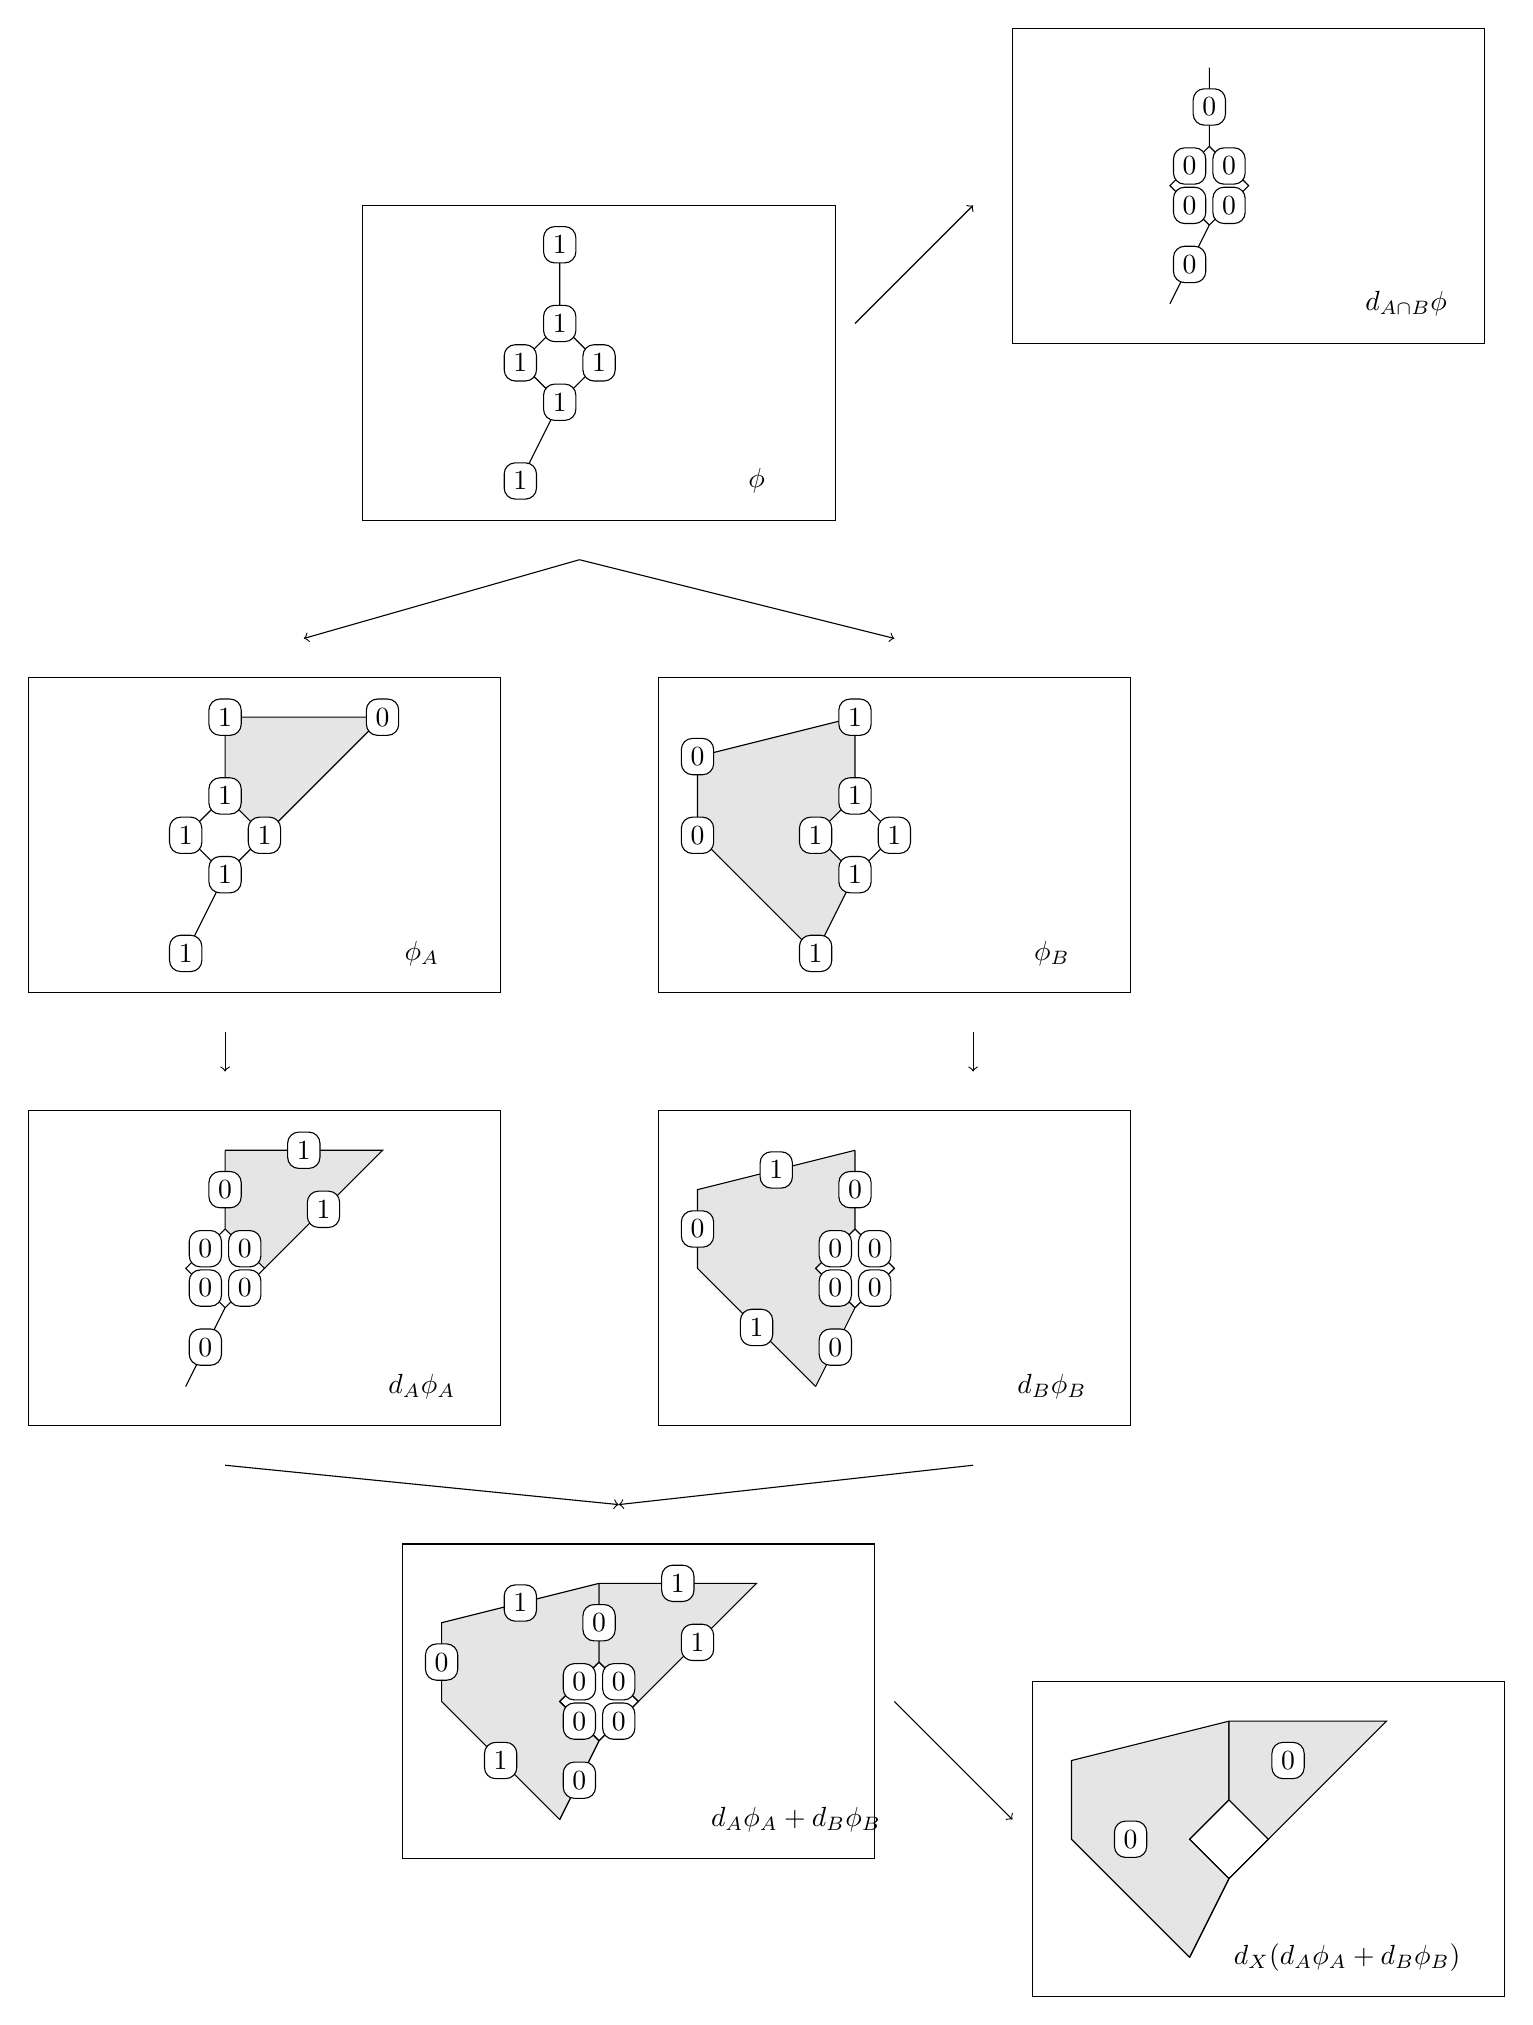
\begin{tikzpicture}

	\begin{scope}[shift={(-6.75,13.5)}]
	\draw (1,1.5) -- (1,0.5) -- (0.5,0) -- (1,-0.5) -- (1.5,0) -- (1,0.5) (1,-0.5) -- (0.5,-1.5);
	\node[draw, fill=white, rounded corners] at (0.5,-1.5) {1};
	\node[draw, fill=white, rounded corners] at (1,-0.5) {1};
	\node[draw, fill=white, rounded corners] at (0.5,0) {1};
	\node[draw, fill=white, rounded corners] at (1,0.5) {1};
	\node[draw, fill=white, rounded corners] at (1.5,0) {1};
	\node[draw, fill=white, rounded corners] at (1,1.5) {1};
	\draw  (-1.5,2) rectangle (4.5,-2);
	\node at (3.5,-1.5) {$\phi$};
	\end{scope}
	\begin{scope}[shift={(1.5,15.75)}]
	\draw (1,1.5) -- (1,0.5) -- (0.5,0) -- (1,-0.5) -- (1.5,0) -- (1,0.5) (1,-0.5) -- (0.5,-1.5);
	
	\node[draw, fill=white, rounded corners] at (0.75,-1) {0};
	\node[draw, fill=white, rounded corners] at (0.75,-0.25) {0};
	\node[draw, fill=white, rounded corners] at (1.25,-0.25) {0};
	\node[draw, fill=white, rounded corners] at (0.75,0.25) {0};
	\node[draw, fill=white, rounded corners] at (1.25,0.25) {0};
	\node[draw, fill=white, rounded corners] at (1,1) {0};
	\draw  (-1.5,2) rectangle (4.5,-2);
	\node at (3.5,-1.5) {$d_{A\cap B}\phi$};
	\end{scope}
	
	
	\begin{scope}[shift={(-3,2)}]
	\fill[gray!20] (-1,0) -- (-1,1) -- (1,1.5)-- (1,0.5) -- (0.5,0) -- (1,-0.5) -- (0.5,-1.5) -- cycle;
	
	\draw (1,1.5) -- (1,0.5) -- (0.5,0) -- (1,-0.5) -- (1.5,0) -- (1,0.5) (1,-0.5) -- (0.5,-1.5);
	\draw (0.5,-1.5) -- (-1,0) -- (-1,1) -- (1,1.5);
	\node[draw, fill=white, rounded corners] at (-0.25,-0.75) {1};
	\node[draw, fill=white, rounded corners] at (-1,0.5) {0};
	\node[draw, fill=white, rounded corners] at (0,1.25) {1};
	\node[draw, fill=white, rounded corners] at (1,1) {0};
	\node[draw, fill=white, rounded corners] at (0.75,0.25) {0};
	\node[draw, fill=white, rounded corners] at (0.75,-0.25) {0};
	\node[draw, fill=white, rounded corners] at (1.25,-0.25) {0};
	\node[draw, fill=white, rounded corners] at (1.25,0.25) {0};
	\node[draw, fill=white, rounded corners] at (0.75,-1) {0};
	\draw  (-1.5,2) rectangle (4.5,-2);
	\node at (3.5,-1.5) {$d_B\phi_B$};
	\end{scope}
	
	
	\begin{scope}[shift={(-11,2)}]
	
	\fill[gray!20] (1,0.5) -- (1.5,0) -- (3,1.5) -- (1,1.5) -- cycle;
	\draw (1,1.5) -- (1,0.5) -- (0.5,0) -- (1,-0.5) -- (1.5,0) -- (1,0.5) (1,-0.5) -- (0.5,-1.5);
	\draw (1,1.5) -- (3,1.5) -- (1.5,0);
	\node[draw, fill=white, rounded corners] at (1,1) {0};
	\node[draw, fill=white, rounded corners] at (1.25,0.25) {0};
	\node[draw, fill=white, rounded corners] at (0.75,0.25) {0};
	\node[draw, fill=white, rounded corners] at (0.75,-0.25) {0};
	\node[draw, fill=white, rounded corners] at (1.25,-0.25) {0};
	\node[draw, fill=white, rounded corners] at (0.75,-1) {0};
	\node[draw, fill=white, rounded corners] at (2.25,0.75) {1};
	\node[draw, fill=white, rounded corners] at (2,1.5) {1};
	\draw  (-1.5,2) rectangle (4.5,-2);
	\node at (3.5,-1.5) {$d_A\phi_A$};
	\end{scope}
	
	
	\begin{scope}[shift={(-3,7.5)}]
	\fill[gray!20] (-1,0) -- (-1,1) -- (1,1.5)-- (1,0.5) -- (0.5,0) -- (1,-0.5) -- (0.5,-1.5) -- cycle;
	
	\draw (1,1.5) -- (1,0.5) -- (0.5,0) -- (1,-0.5) -- (1.5,0) -- (1,0.5) (1,-0.5) -- (0.5,-1.5);
	\draw (0.5,-1.5) -- (-1,0) -- (-1,1) -- (1,1.5);
	\node[draw, fill=white, rounded corners] at (0.5,-1.5) {1};
	\node[draw, fill=white, rounded corners] at (1,-0.5) {1};
	\node[draw, fill=white, rounded corners] at (0.5,0) {1};
	\node[draw, fill=white, rounded corners] at (1,0.5) {1};
	\node[draw, fill=white, rounded corners] at (1.5,0) {1};
	\node[draw, fill=white, rounded corners] at (1,1.5) {1};
	\node[draw, fill=white, rounded corners] at (-1,0) {0};
	\node[draw, fill=white, rounded corners] at (-1,1) {0};
	\draw  (-1.5,2) rectangle (4.5,-2);
	\node at (3.5,-1.5) {$\phi_B$};
	\end{scope}
	
	
	\begin{scope}[shift={(-11,7.5)}]
	
	\fill[gray!20] (1,0.5) -- (1.5,0) -- (3,1.5) -- (1,1.5) -- cycle;
	\draw (1,1.5) -- (1,0.5) -- (0.5,0) -- (1,-0.5) -- (1.5,0) -- (1,0.5) (1,-0.5) -- (0.5,-1.5);
	\draw (1,1.5) -- (3,1.5) -- (1.5,0);
	\node[draw, fill=white, rounded corners] at (0.5,-1.5) {1};
	\node[draw, fill=white, rounded corners] at (1,-0.5) {1};
	\node[draw, fill=white, rounded corners] at (0.5,0) {1};
	\node[draw, fill=white, rounded corners] at (1,0.5) {1};
	\node[draw, fill=white, rounded corners] at (1.5,0) {1};
	\node[draw, fill=white, rounded corners] at (1,1.5) {1};
	\node[draw, fill=white, rounded corners] at (3,1.5) {0};
	\draw  (-1.5,2) rectangle (4.5,-2);
	\node at (3.5,-1.5) {$\phi_A$};
	\end{scope}
	
	
	
	\begin{scope}[shift={(-6.25,-3.5)}]
	\fill[gray!20] (-1,0) -- (-1,1) -- (1,1.5)-- (1,0.5) -- (0.5,0) -- (1,-0.5) -- (0.5,-1.5) -- cycle;
	
	\draw (1,1.5) -- (1,0.5) -- (0.5,0) -- (1,-0.5) -- (1.5,0) -- (1,0.5) (1,-0.5) -- (0.5,-1.5);
	\draw (0.5,-1.5) -- (-1,0) -- (-1,1) -- (1,1.5);
	\node[draw, fill=white, rounded corners] at (-0.25,-0.75) {1};
	\node[draw, fill=white, rounded corners] at (-1,0.5) {0};
	\node[draw, fill=white, rounded corners] at (0,1.25) {1};
	
	\fill[gray!20] (1,0.5) -- (1.5,0) -- (3,1.5) -- (1,1.5) -- cycle;
	\draw (1,1.5) -- (1,0.5) -- (0.5,0) -- (1,-0.5) -- (1.5,0) -- (1,0.5) (1,-0.5) -- (0.5,-1.5);
	\draw (1,1.5) -- (3,1.5) -- (1.5,0);
	\node[draw, fill=white, rounded corners] at (1,1) {0};
	\node[draw, fill=white, rounded corners] at (1.25,0.25) {0};
	\node[draw, fill=white, rounded corners] at (0.75,0.25) {0};
	\node[draw, fill=white, rounded corners] at (0.75,-0.25) {0};
	\node[draw, fill=white, rounded corners] at (1.25,-0.25) {0};
	\node[draw, fill=white, rounded corners] at (0.75,-1) {0};
	\node[draw, fill=white, rounded corners] at (2.25,0.75) {1};
	\node[draw, fill=white, rounded corners] at (2,1.5) {1};
	\draw  (-1.5,2) rectangle (4.5,-2);
	
	\node at (3.5,-1.5) {$d_A\phi_A+d_B\phi_B$};
	\end{scope}
	
	
	\begin{scope}[shift={(1.75,-5.25)}]
	\fill[gray!20] (-1,0) -- (-1,1) -- (1,1.5)-- (1,0.5) -- (0.5,0) -- (1,-0.5) -- (0.5,-1.5) -- cycle;
	
	\draw (1,1.5) -- (1,0.5) -- (0.5,0) -- (1,-0.5) -- (1.5,0) -- (1,0.5) (1,-0.5) -- (0.5,-1.5);
	\draw (0.5,-1.5) -- (-1,0) -- (-1,1) -- (1,1.5);
	\fill[gray!20] (1,0.5) -- (1.5,0) -- (3,1.5) -- (1,1.5) -- cycle;
	\draw (1,1.5) -- (1,0.5) -- (0.5,0) -- (1,-0.5) -- (1.5,0) -- (1,0.5) (1,-0.5) -- (0.5,-1.5);
	\draw (1,1.5) -- (3,1.5) -- (1.5,0);
	\node[draw, fill=white, rounded corners] at (-0.25,0) {0};
	\node[draw, fill=white, rounded corners] at (1.75,1) {0};
	\draw  (-1.5,2) rectangle (4.5,-2);
	\node at (2.5,-1.5) {$d_X (d_A\phi_A+d_B\phi_B)$};
	\end{scope}
	
	\draw[->] (-5.5,11) -- (-9,10);
	\draw[->] (-5.5,11) -- (-1.5,10);
	\draw[->] (-10,5) -- (-10,4.5);
	\draw[->] (-0.5,5) -- (-0.5,4.5);
	\draw[->] (-10,-0.5) -- (-5,-1);
	\draw[->] (-0.5,-0.5) -- (-5,-1);
	\draw[->] (-1.5,-3.5) -- (0,-5);
	\draw[->] (-2,14) -- (-0.5,15.5);
	\end{tikzpicture}}\]



\begin{doubledpage}{example}{Homology of Sphere}
	{Let's compute the homology of sphere $S^n$ by using Mayer-Vietoris and induction. For this example, we will start with the assumptions that we know the homology of a disk \ref{exam:diskhomology}.}
	 We will prove that $H^k(S^n)=\ZZ_2$ if and only if $k=n, 0$ by induction on $n$.  
	Here, we will run the Mayer-Vietoris argument on a the decomposition of $S^n$ into two disks, $A, B= D^n$, which are suppose to represent the upper and lower hemispheres. Notice that the intersection of the two hemispheres is the equatorial sphere, which is a sphere of 1-dimension lower.
	\[\begin{tikzpicture}[scale=.4]
      \newcommand{\vertexradius}{2.5pt}
\newcommand{\vertexscale}{.5}
\newcommand{\bigvertexscale}{1}
\newcommand{\vertex}{\node[circle, fill=black, scale=\vertexscale] }
\newcommand{\highlighta}{red!20}
\newcommand{\highlightb}{blue!20}
\newcommand{\highlightc}{green!20}
\newcommand{\shadinga}{gray!20}
\newcommand{\smallvertex}{\node[circle, fill=black, scale=.2]}
\newcommand{\highlightlinewidth}{3pt}

\tikzset{every path/.style={line width=1 pt}}

\begin{scope}[shift={(-6,4)}]
\fill[gray!20] (0,-1) ellipse (1 and .3);
\draw  (-2,1) rectangle (3,-3);
\begin{scope}[]
\clip  (-2,0) rectangle (2,-1);
\draw[dashed]  (0,-1) ellipse (1 and .3);
\end{scope}
\begin{scope}[]
\clip  (2,-2) rectangle (-2,-1);
\draw[fill=gray!20]  (0,-1) ellipse (1 and 1);
\draw (0,-1) ellipse (1 and .3);
\end{scope}
\node at (2,0) {$D^n$};
\end{scope}



\begin{scope}[shift={(-6,-2)}]
\draw  (-2,1) rectangle (3,-3);
\fill[gray!20] (0,-1) ellipse (1 and .3);
\begin{scope}[]
\clip  (-2,0) rectangle (2,-1);
\draw[fill=gray!20]  (0,-1) ellipse (1 and 1);
\draw[dashed]  (0,-1) ellipse (1 and .3);
\end{scope}
\begin{scope}[]
\clip  (2,-2) rectangle (-2,-1);
\draw (0,-1) ellipse (1 and .3);
\end{scope}
\node at (2,0) {$D^n$};
\end{scope}

\begin{scope}[shift={(-14,1)}]
\draw  (-2,1) rectangle (3,-3);
\draw (0,-1) ellipse (1 and .3);

\node at (2,0) {$S^{n-1}$};
\end{scope}\begin{scope}[shift={(2,1)}]
\draw  (-2,1) rectangle (3,-3);
\draw[fill=gray!20]  (0,-1) ellipse (1 and 1);
\begin{scope}[]
\clip  (-2,0) rectangle (2,-1);
\draw[dashed]  (0,-1) ellipse (1 and .3);
\end{scope}
\begin{scope}[]
\clip  (2,-2) rectangle (-2,-1);
\draw (0,-1) ellipse (1 and .3);
\end{scope}
\node at (2,0) {$S^n$};
\end{scope}
\draw[->] (-10,1) -- (-9,3);
\draw[->] (-10,-1) -- (-9,-3);
\draw[->] (-2,3) -- (-1,1);
\draw[->] (-2,-3) -- (-1,-1);
\pgfsize 
\end{tikzpicture}\]
	 So, we have a short exact sequence of chain complexes:
	\[0\to C^\bullet(S^{n})\to C^\bullet(D^n)\oplus C^\bullet(D^n)\to C_\bullet(S^{n-1})\to 0\]
	This short exact sequence gives us a long exact sequence of homology groups :
		\[
			\begin{tikzcd}
				H^{0  }(S^{n}) \arrow{r}\arrow[draw=none]{d}[name=Z, shape=coordinate]{}&H^{0}  (D^n)\oplus H^{0  }(D^n)  \arrow{r}& H^{0  }    (S^{n-1}) \arrow[rounded corners,to path={ -- ([xshift=2ex]\tikztostart.east)|- (Z) [near end]\tikztonodes-| ([xshift=-2ex]\tikztotarget.west)-- (\tikztotarget)}]{dll}{\delta} \\
				H^{1  }(S^{n}) \arrow{r}\arrow[draw=none]{d}[name=Z, shape=coordinate]{}&H^{1}  (D^n)\oplus H^{1  }(D^n)  \arrow{r}& H^{1  }    (S^{n-1}) \arrow[rounded corners,to path={ -- ([xshift=2ex]\tikztostart.east)|- (Z) [near end]\tikztonodes-| ([xshift=-2ex]\tikztotarget.west)-- (\tikztotarget)}]{dll}{\delta} \\
				H^{2  }(S^{n}) \arrow{r}\arrow[draw=none]{d}[name=Z, shape=coordinate]{}&\cdots 					      \arrow{r}& H^{n-2}    (S^{n-1}) \arrow[rounded corners,to path={ -- ([xshift=2ex]\tikztostart.east)|- (Z) [near end]\tikztonodes-| ([xshift=-2ex]\tikztotarget.west)-- (\tikztotarget)}]{dll}{\delta} \\
				H^{n-1}(S^{n}) \arrow{r}\arrow[draw=none]{d}[name=Z, shape=coordinate]{}&H^{n-1}(D^n)\oplus H^{n-1}(D^n)  \arrow{r}& H^{n-1}    (S^{n-1}) \arrow[rounded corners,to path={ -- ([xshift=2ex]\tikztostart.east)|- (Z) [near end]\tikztonodes-| ([xshift=-2ex]\tikztotarget.west)-- (\tikztotarget)}]{dll}{\delta} \\
				H^{n  }(S^{n}) \arrow{r}{i_0\oplus j_0 }								&H^{n  }(D^n)\oplus H^{n  }(D^n)  \arrow{r}& H^{n  }    (S^{n-1}) \arrow{r}&0
			\end{tikzcd}
	\]
	Substituting in the groups we know from induction and our assumptions
		\[
			\begin{tikzcd}
				H^{0  }(S^{n}) \arrow{r}\arrow[draw=none]{d}[name=Z, shape=coordinate]{}&  \ZZ_2\oplus \ZZ_2    \arrow{r}& \ZZ_2    \arrow[rounded corners,to path={ -- ([xshift=2ex]\tikztostart.east)|- (Z) [near end]\tikztonodes-| ([xshift=-2ex]\tikztotarget.west)-- (\tikztotarget)}]{dll}{\delta} \\
				H^{1  }(S^{n}) \arrow{r}\arrow[draw=none]{d}[name=Z, shape=coordinate]{}& 0                     \arrow{r}& 0            \arrow[rounded corners,to path={ -- ([xshift=2ex]\tikztostart.east)|- (Z) [near end]\tikztonodes-| ([xshift=-2ex]\tikztotarget.west)-- (\tikztotarget)}]{dll}{\delta} \\
				H^{2  }(S^{n}) \arrow{r}\arrow[draw=none]{d}[name=Z, shape=coordinate]{}& \cdots                \arrow{r}& 0            \arrow[rounded corners,to path={ -- ([xshift=2ex]\tikztostart.east)|- (Z) [near end]\tikztonodes-| ([xshift=-2ex]\tikztotarget.west)-- (\tikztotarget)}]{dll}{\delta} \\
				H^{n-1}(S^{n}) \arrow{r}\arrow[draw=none]{d}[name=Z, shape=coordinate]{}& 0                     \arrow{r}& \ZZ_2        \arrow[rounded corners,to path={ -- ([xshift=2ex]\tikztostart.east)|- (Z) [near end]\tikztonodes-| ([xshift=-2ex]\tikztotarget.west)-- (\tikztotarget)}]{dll}{\delta} \\
				H^{n  }(S^{n}) \arrow{r}{i_0\oplus j_0 }                                &    0                  \arrow{r}& 0\arrow{r}&0
			\end{tikzcd}
	\]
	We therefore may now look at these shorter exact sequences instead:
	\[0\to  \ZZ_2\to H^n(S^n)\to 0\]
	\[0\to H^k(S^n) \to 0 \;\;\;\;\;\;\;\; k\neq n, 0\]
	\[0\to H^0(S^n)\to Z_2\oplus Z_2\to Z_2\to H^1(S^n)\to 0\]
	Running through the properties of exactness at each part shows confirms our computation of the homology of $S^n$. 
	\end{doubledpage}

\begin{elevator}[Inclusion-Exclusion principles: The Zig-Zag Lemma]
\label{append:inexzigzag}
Let's now use Inclusion-Exclusion to build up some more intuition on what homological algebra can get us. We will now work a little abstractly.
\end{elevator}
Let $\mathcal C$ be a collection of objects. Let's suppose that objects in this collection admit decompositions, so that we may write \footnote{We also adopt homological grading conventions in this section, as opposed to cohomological grading conditions. }
\[X=A\cup B\]
and for every such decomposition, we may also associate an objects called $A\cap B$. 

A \emph{property} is a function $P: \mathcal C\to \N$ which assigns to each object a number. 
%\begin{example}
%Let our group of objects be $\Set$, the set of all finite sets. Then given $f: A\to X$, and $g: B\to X$, we have that $X=A\cup B$ if the map $f\sqcup g: A\sqcup B \to X$ was surjective. \\
%In this case, we can also define $A\cap B$. The property that we're interested in the case of sets is their size, which defines a function $|\;\cdot \;|: \Set \to \N.$
%\end{example}
%\begin{example}
%Let our group of objects be graphs. Similarly we have an idea of covering $G=H_1\cup H_2$, and an idea of intersection.\\
%There are several different properties we could look at. We could look at $|V(G)|$, which measures the number of vertices, or $|E(G)|$, which measures the number of edges. \\
%A more interesting property is the number of connected components, $b_0(G)$, or $b_1(G)$, the dimension of the cycle space.\\
%A very difficult property to compute is $\gamma_G(k)$, which computes the number of $k$-colorings. 
%\end{example}
%Our goal is to come up with a general framework to understand how to compute properties with the framework of decompositions. 
%\begin{definition}
%A category $\mathcal C$ and a property $P$ satisfy an \emph{inclusion-exclusion principle} if for every decomposition $X=A\cup B$, we have 
%\[P(X)=P(A)+P(B)-P(A\cap B).\]
%\end{definition}
%Sets, and sizes of sets is a classic example of a category and a property that obey the inclusion-exclusion principle. However, many properties do not satisfy the inclusion-exclusion principle. 
%\begin{example}
%Let $C_n$ be a cycle, and $C_n=P_{m_1}\cup P_{m_2}$ be a decomposition so that $P_{m_1}\cap P_{m_2}=\{u,v\}. $ Then we have that $b_0(C_n)=1$, but 
%\[b_0(P_{m_1})+b_0(P_{m_2})-b_0(P_{m_1}\cap P_{m_2})=0.\]
%This property does not have the inclusion-exclusion property
%\end{example}
%Though the inclusion-exclusion property does not hold, it almost holds, and the more subtle properties of graphs is what prevents the inclusion-exclusion properties from holding. However, we can access some of these properties by using homological algebra. 
\begin{definition}
Let $\mathcal C$ be a category, and $P: \mathcal C\to \N$ be a property. We say that $P$ obeys the \emph{homological inclusion-exclusion principle} if for all $X$, there exists a chain complex $P_\bullet(X)$ satisfying the following conditions:
\begin{itemize}
\item \emph{Recovery of $P$:} We have that $\dim H_0(P_\bullet(X))=P(X).$
\item \emph{Inclusion-Exclusion:} Whenever $X=A\cup B$, we have a short exact sequence:
\[0\to P_\bullet(A\cap B)\to P_\bullet(A)\oplus P_\bullet(B)\to P_\bullet(X)\to 0.\]
\end{itemize}
\end{definition}
Notice that satisfying a homological inclusion-exclusion principle is in a lot of ways like satisfying a inclusion-exclusion principle, in that 
\[\dim(P_0(X))= \dim (P_0(A))+\dim(P_0(B))-\dim(P_0(A\cap B)).\]
While we don't get an actual inclusion exclusion principle from a homological inclusion-exclusion principle, we get something very close to the principle holding. In order to see the relation between inclusion-exclusion and homological inclusion-exclusion, we need a powerful lemma from homological algebra. 
\begin{theorem}[Zig-Zag Lemma]
Let $ A_\bullet,\partial^A_\bullet$ , $ B_\bullet,d^B_\bullet$ and $C_\bullet,d^C_\bullet$ be chain complexes. Given 
\[\begin{tikzcd} 0\arrow{r}&  A_\bullet \arrow{r}{f}& B_\bullet \arrow{r}{g} &C_\bullet \arrow{r} &0\end{tikzcd}\] a short exact sequence, there exists a unique map $\delta$ such that the following is a long exact sequence on homology:
\[\begin{tikzcd}[column sep=small] \cdots \arrow{r}{g_*}&H_{n+1}(C)\arrow{r}{\delta}& H_n ( A)\arrow{r}{f_*}& H_n( B)\arrow{r}{g_*}& H_n(C)\arrow{r}{\delta}& H_{n-1}( A)\arrow{r}{f_*}&\cdots \end{tikzcd}\] \label{lemma:zigzag}
\end{theorem}
Before we get into a proof of this theorem, let's quickly make a remark on the map $\delta$. On the one hand, the map is remarkable, as there is no reason to expect a map connecting $C\to A$. However, we've seen the existence of a long exact sequence that arises from a short exact sequence before when we looked at cones. \\
\begin{projectdescription}{Foo}
In a certain sense, this theorem says that \emph{all short exact sequences of chain complexes essentially arise from the cone sequence.} While we will not be able to prove this result in this class, one can make a version of this statement true by exploring the derived category and triangulated structures.  \label{proj:derived}
\end{projectdescription}
\begin{proof}
First, let's expand the original diagram:
\[\begin{tikzcd}
\; & \vdots   \arrow{d}{\partial} & \vdots\arrow{d}{\partial^B} &\vdots \arrow{d}{\partial^C}&\\
0\arrow{r}& A_{n+1}\arrow{d}{\partial_{n+1}}\arrow{r}{f_{n+1}} & B_{n+1}\arrow{d}{\partial^B_{n+1}}\arrow{r}{g_{n+1}} & C_{n+1}\arrow{d}{\partial^C_{n+1}}\arrow{r}&0\\
0\arrow{r}& A_{n  }\arrow{d}{\partial^A_{n  }}\arrow{r}{f_{n  }} & B_{n  }\arrow{d}{\partial^B_{n  }}\arrow{r}{g_{n  }} & C_{n  }\arrow{d}{\partial^C_{n  }}\arrow{r}&0\\
0\arrow{r}& A_{n-1}\arrow{d}{\partial^A_{n-1}}\arrow{r}{f_{n-1}} & B_{n-1}\arrow{d}{\partial^B_{n-1}}\arrow{r}{g_{n-1}} & C_{n-1}\arrow{d}{\partial^C_{n-1}}\arrow{r}&0\\
\;&\vdots&\vdots&\vdots&
\end{tikzcd}\]
We want to construct a function $\delta$ from $H_{n}(C)$ to $H_{n-1}(A)$. The following argument is an \emph{element chasing argument}, which can be a bit difficult to follow through; it's suggested that the reader write out the argument step-by-step at some point on their own to see where the maps come from.\\
Since this lemma contains several statements, we will check some of them and leave the remainder as exercises. 
\begin{claim}
There exists a canonical map $\delta: H_k(C)\to H_{k-1}(A).$
\end{claim}
As mentioned before, we should somewhat expect the existence of this map from our studies of cones. First, let's try and show that to a homology class $[\gamma]\in H_k(C)$, we can find an element in $A_{k-1}$  
\begin{itemize}
\item As the map $g_n$ is surjective, we know that we can pick an element in the preimage $\beta$ so that $g_n(\beta)=\gamma$. \emph{Notice that this is not a canonical choice!}
\[ 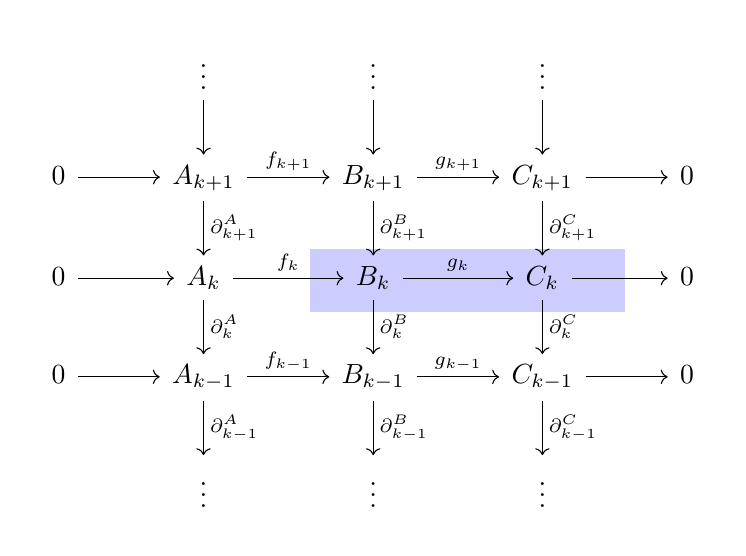
\begin{tikzpicture}
\usetikzlibrary{cd}


\fill[fill=blue!20]  (-0.8,3.2) rectangle (3.2,2.4);

\matrix[matrix of math nodes, name=m, commutative diagrams/every cell, row sep= 20, column sep = 30] {
\; & \vdots   & \vdots&\vdots &\\
0& A_{k+1} & B_{k+1} & C_{k+1}&0\\
0& A_{k} & B_{k} & C_{k}&0\\
0& A_{k-1} & B_{k-1} & C_{k-1}&0\\
\;&\vdots &\vdots &\vdots &\\};
\path[commutative diagrams/.cd, every arrow, every label]
(m-1-2) edge (m-2-2)    (m-1-3) edge (m-2-3)     (m-1-4) edge (m-2-4)
(m-2-1) edge (m-2-2)
(m-2-2) edge node {$\partial^A_{k+1}$} (m-3-2)    edge node {$f_{k+1}$} (m-2-3)      
(m-2-3)edge node {$\partial^B_{k+1}$} (m-3-3)    edge node {$g_{k+1}$}  (m-2-4)  
(m-2-4) edge node {$\partial^C_{k+1}$}(m-3-4)  edge (m-2-5)  

(m-3-1) edge (m-3-2)
(m-3-2) edge node {$\partial^A_{k}$} (m-4-2)    edge node {$f_{k}$} (m-3-3)      
(m-3-3)edge node {$\partial^B_{k}$} (m-4-3)    edge node {$g_{k}$}  (m-3-4)  
(m-3-4) edge node {$\partial^C_{k}$}(m-4-4)  edge (m-3-5)  

(m-4-1) edge (m-4-2)
(m-4-2) edge node {$\partial^A_{k-1}$} (m-5-2)    edge node {$f_{k-1}$} (m-4-3)      
(m-4-3)edge node {$\partial^B_{k-1}$} (m-5-3)    edge node {$g_{k-1}$}  (m-4-4)  
(m-4-4) edge node {$\partial^C_{k-1}$}(m-5-4)  edge (m-4-5)  
;
\end{tikzpicture}\]
\item We can apply $\partial^B_n(\beta)$ and we wind up with an element in $B_{n-1}$. Using that $g_{n-1}$ is a chain map, we get that  
\[g_{n-1} \partial^B_n(\beta)= \partial^Cg_n(\beta)=\partial^C \gamma =0\]
where the second equality comes from the fact that $\gamma$ represents a homology class. 
\[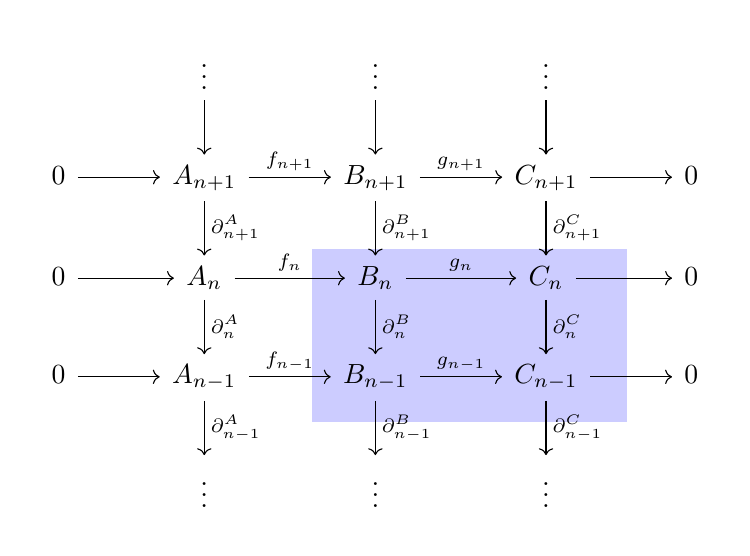
\begin{tikzpicture}
\usetikzlibrary{cd}

\fill[fill=blue!20]  (-0.8,3.2) rectangle (3.2,1);
\matrix[matrix of math nodes, name=m, commutative diagrams/every cell, row sep= 20, column sep = 30] {
\; & \vdots   & \vdots&\vdots &\\
0& A_{n+1} & B_{n+1} & C_{n+1}&0\\
0& A_{n} & B_{n} & C_{n}&0\\
0& A_{n-1} & B_{n-1} & C_{n-1}&0\\
\;&\vdots &\vdots &\vdots &\\};
\path[commutative diagrams/.cd, every arrow, every label]
(m-1-2) edge (m-2-2)    (m-1-3) edge (m-2-3)     (m-1-4) edge (m-2-4)
(m-2-1) edge (m-2-2)
(m-2-2) edge node {$\partial^A_{n+1}$} (m-3-2)    edge node {$f_{n+1}$} (m-2-3)      
(m-2-3)edge node {$\partial^B_{n+1}$} (m-3-3)    edge node {$g_{n+1}$}  (m-2-4)  
(m-2-4) edge node {$\partial^C_{n+1}$}(m-3-4)  edge (m-2-5)  

(m-3-1) edge (m-3-2)
(m-3-2) edge node {$\partial^A_{n}$} (m-4-2)    edge node {$f_{n}$} (m-3-3)      
(m-3-3)edge node {$\partial^B_{n}$} (m-4-3)    edge node {$g_{n}$}  (m-3-4)  
(m-3-4) edge node {$\partial^C_{n}$}(m-4-4)  edge (m-3-5)  

(m-4-1) edge (m-4-2)
(m-4-2) edge node {$\partial^A_{n-1}$} (m-5-2)    edge node {$f_{n-1}$} (m-4-3)      
(m-4-3)edge node {$\partial^B_{n-1}$} (m-5-3)    edge node {$g_{n-1}$}  (m-4-4)  
(m-4-4) edge node {$\partial^C_{n-1}$}(m-5-4)  edge (m-4-5)  
;
\end{tikzpicture}\]
\item Since $\partial^B_n(\beta)\in \ker g_{n-}1$, and the sequence is chain complexes is exact, we know that $\partial^B_(\beta)\in \im f_{n-1}$. Since $f_{n-1}$ is injective, we know that there is unique $\alpha$ corresponding to this $\beta$ so that $f_{n-1}(\alpha)=\partial^B(\beta).$
\[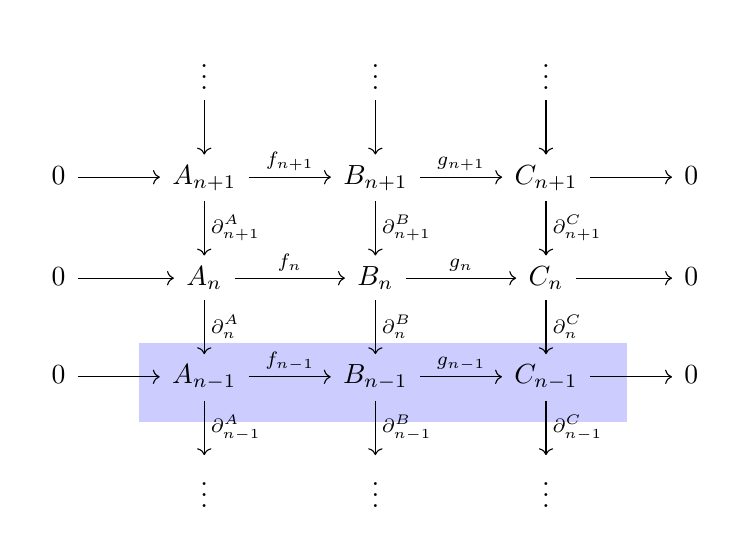
\begin{tikzpicture}
\usetikzlibrary{cd}


\fill[fill=blue!20]  (-3,2) rectangle (3.2,1);

\matrix[matrix of math nodes, name=m, commutative diagrams/every cell, row sep= 20, column sep = 30] {
\; & \vdots   & \vdots&\vdots &\\
0& A_{n+1} & B_{n+1} & C_{n+1}&0\\
0& A_{n} & B_{n} & C_{n}&0\\
0& A_{n-1} & B_{n-1} & C_{n-1}&0\\
\;&\vdots &\vdots &\vdots &\\};
\path[commutative diagrams/.cd, every arrow, every label]
(m-1-2) edge (m-2-2)    (m-1-3) edge (m-2-3)     (m-1-4) edge (m-2-4)
(m-2-1) edge (m-2-2)
(m-2-2) edge node {$\partial^A_{n+1}$} (m-3-2)    edge node {$f_{n+1}$} (m-2-3)      
(m-2-3)edge node {$\partial^B_{n+1}$} (m-3-3)    edge node {$g_{n+1}$}  (m-2-4)  
(m-2-4) edge node {$\partial^C_{n+1}$}(m-3-4)  edge (m-2-5)  

(m-3-1) edge (m-3-2)
(m-3-2) edge node {$\partial^A_{n}$} (m-4-2)    edge node {$f_{n}$} (m-3-3)      
(m-3-3)edge node {$\partial^B_{n}$} (m-4-3)    edge node {$g_{n}$}  (m-3-4)  
(m-3-4) edge node {$\partial^C_{n}$}(m-4-4)  edge (m-3-5)  

(m-4-1) edge (m-4-2)
(m-4-2) edge node {$\partial^A_{n-1}$} (m-5-2)    edge node {$f_{n-1}$} (m-4-3)      
(m-4-3)edge node {$\partial^B_{n-1}$} (m-5-3)    edge node {$g_{n-1}$}  (m-4-4)  
(m-4-4) edge node {$\partial^C_{n-1}$}(m-5-4)  edge (m-4-5)  
;
\end{tikzpicture}\]
\item We initially define $\delta[\gamma]=\alpha$. 
\end{itemize}
We now need to show that $\alpha$ is a homology class, that is, that $\partial_{k-1}^A(\alpha)=0$. 
\begin{itemize}
\item Look at $\partial_{k-1}^A(\alpha)$. Since this diagram is commutative, we have that $f_{k-2} \partial^A_{k-1}(\alpha)= \partial^B_{k-1}f_{k-1}(\alpha).$
\[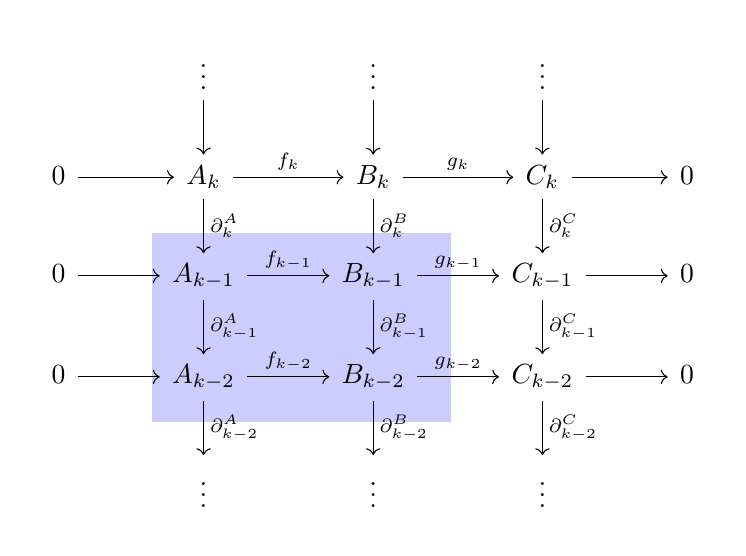
\begin{tikzpicture}
\usetikzlibrary{cd}


\fill[fill=blue!20]  (-2.8,3.4) rectangle (1,1);

\matrix[matrix of math nodes, name=m, commutative diagrams/every cell, row sep= 20, column sep = 30] {
\; & \vdots   & \vdots&\vdots &\\
0& A_{k} & B_{k} & C_{k}&0\\
0& A_{k-1} & B_{k-1} & C_{k-1}&0\\
0& A_{k-2} & B_{k-2} & C_{k-2}&0\\
\;&\vdots &\vdots &\vdots &\\};
\path[commutative diagrams/.cd, every arrow, every label]
(m-1-2) edge (m-2-2)    (m-1-3) edge (m-2-3)     (m-1-4) edge (m-2-4)
(m-2-1) edge (m-2-2)
(m-2-2) edge node {$\partial^A_{k}$} (m-3-2)    edge node {$f_{k}$} (m-2-3)      
(m-2-3)edge node {$\partial^B_{k}$} (m-3-3)    edge node {$g_{k}$}  (m-2-4)  
(m-2-4) edge node {$\partial^C_{k}$}(m-3-4)  edge (m-2-5)  

(m-3-1) edge (m-3-2)
(m-3-2) edge node {$\partial^A_{k-1}$} (m-4-2)    edge node {$f_{k-1}$} (m-3-3)      
(m-3-3)edge node {$\partial^B_{k-1}$} (m-4-3)    edge node {$g_{k-1}$}  (m-3-4)  
(m-3-4) edge node {$\partial^C_{k-1}$}(m-4-4)  edge (m-3-5)  

(m-4-1) edge (m-4-2)
(m-4-2) edge node {$\partial^A_{k-2}$} (m-5-2)    edge node {$f_{k-2}$} (m-4-3)      
(m-4-3)edge node {$\partial^B_{k-2}$} (m-5-3)    edge node {$g_{k-2}$}  (m-4-4)  
(m-4-4) edge node {$\partial^C_{k-2}$}(m-5-4)  edge (m-4-5)  
;
\end{tikzpicture}\]
\item Recalling or definition of $\alpha$, we know that $f_{k-1}(\alpha)= \partial^B_{k}(\beta)$, so $\partial_{k-1}^B(\partial^B_k(\beta)= f_{k-2}(\partial_{k-1}\alpha)=0$. Since $f_{k-2}$ is injective, we get that $\partial_{k-1}\alpha)=0$. 
\[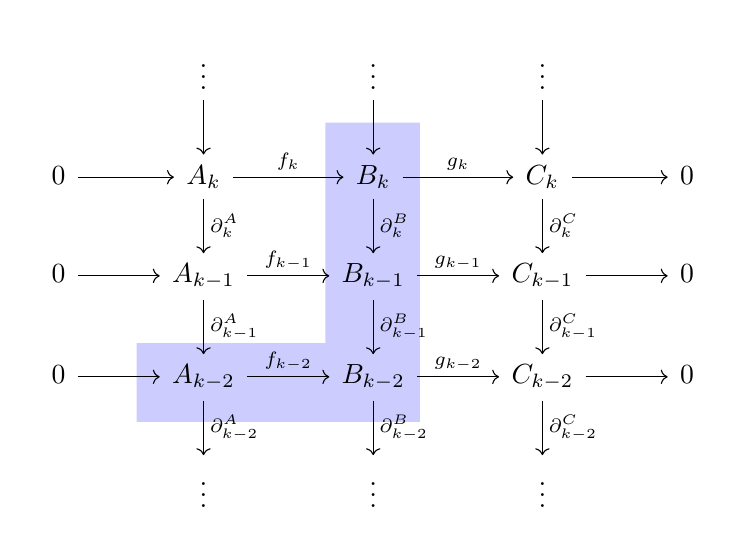
\begin{tikzpicture}
\usetikzlibrary{cd}


\fill[blue!20] (-3,2) -- (-3,1) -- (0.6,1) -- (0.6,4.8) -- (-0.6,4.8) -- (-0.6,2) -- cycle;

\matrix[matrix of math nodes, name=m, commutative diagrams/every cell, row sep= 20, column sep = 30] {
\; & \vdots   & \vdots&\vdots &\\
0& A_{k} & B_{k} & C_{k}&0\\
0& A_{k-1} & B_{k-1} & C_{k-1}&0\\
0& A_{k-2} & B_{k-2} & C_{k-2}&0\\
\;&\vdots &\vdots &\vdots &\\};
\path[commutative diagrams/.cd, every arrow, every label]
(m-1-2) edge (m-2-2)    (m-1-3) edge (m-2-3)     (m-1-4) edge (m-2-4)
(m-2-1) edge (m-2-2)
(m-2-2) edge node {$\partial^A_{k}$} (m-3-2)    edge node {$f_{k}$} (m-2-3)      
(m-2-3)edge node {$\partial^B_{k}$} (m-3-3)    edge node {$g_{k}$}  (m-2-4)  
(m-2-4) edge node {$\partial^C_{k}$}(m-3-4)  edge (m-2-5)  

(m-3-1) edge (m-3-2)
(m-3-2) edge node {$\partial^A_{k-1}$} (m-4-2)    edge node {$f_{k-1}$} (m-3-3)      
(m-3-3)edge node {$\partial^B_{k-1}$} (m-4-3)    edge node {$g_{k-1}$}  (m-3-4)  
(m-3-4) edge node {$\partial^C_{k-1}$}(m-4-4)  edge (m-3-5)  

(m-4-1) edge (m-4-2)
(m-4-2) edge node {$\partial^A_{k-2}$} (m-5-2)    edge node {$f_{k-2}$} (m-4-3)      
(m-4-3)edge node {$\partial^B_{k-2}$} (m-5-3)    edge node {$g_{k-2}$}  (m-4-4)  
(m-4-4) edge node {$\partial^C_{k-2}$}(m-5-4)  edge (m-4-5)  
;
\end{tikzpicture}\]
\end{itemize}
Finally, when we constructed the class $\alpha$, we had to make a choice of $\beta=g_k^{-1}(\gamma)$. Let's show that the homology class of $\alpha$ does not depend on the choice of $\beta$ lifting $\alpha$. 
\begin{itemize}
\item Suppose that $\beta, \beta'$ are two different liftings of $\gamma$ so that $g_k(\beta)-g_k(\beta')=0$. We want to show that the associated classes $[\alpha], [\alpha']$ are homologous. Since $g_k(\beta-\beta')=0$, there exists a class $f_k^{-1}(\beta-\beta')$ due to exactness of the row. 
 \[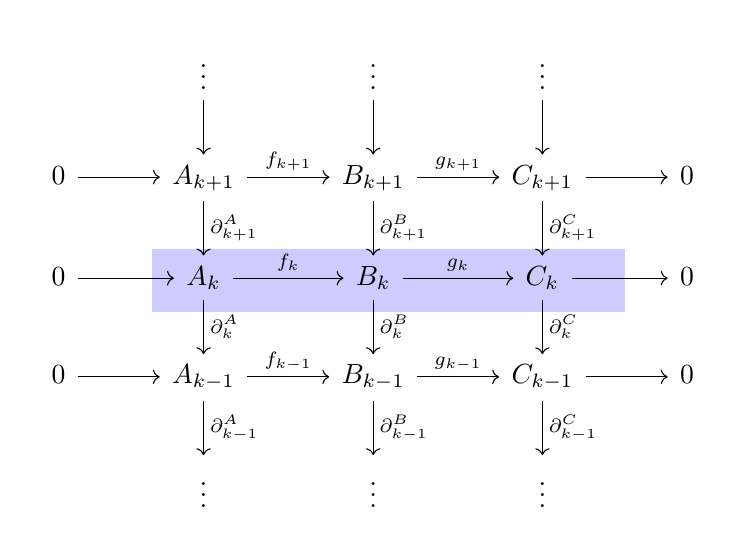
\begin{tikzpicture}
\usetikzlibrary{cd}
\fill[fill=blue!20]  (-2.8,3.2) rectangle (3.2,2.4);

\matrix[matrix of math nodes, name=m, commutative diagrams/every cell, row sep= 20, column sep = 30] {
\; & \vdots   & \vdots&\vdots &\\
0& A_{k+1} & B_{k+1} & C_{k+1}&0\\
0& A_{k} & B_{k} & C_{k}&0\\
0& A_{k-1} & B_{k-1} & C_{k-1}&0\\
\;&\vdots &\vdots &\vdots &\\};
\path[commutative diagrams/.cd, every arrow, every label]
(m-1-2) edge (m-2-2)    (m-1-3) edge (m-2-3)     (m-1-4) edge (m-2-4)
(m-2-1) edge (m-2-2)
(m-2-2) edge node {$\partial^A_{k+1}$} (m-3-2)    edge node {$f_{k+1}$} (m-2-3)      
(m-2-3)edge node {$\partial^B_{k+1}$} (m-3-3)    edge node {$g_{k+1}$}  (m-2-4)  
(m-2-4) edge node {$\partial^C_{k+1}$}(m-3-4)  edge (m-2-5)  

(m-3-1) edge (m-3-2)
(m-3-2) edge node {$\partial^A_{k}$} (m-4-2)    edge node {$f_{k}$} (m-3-3)      
(m-3-3)edge node {$\partial^B_{k}$} (m-4-3)    edge node {$g_{k}$}  (m-3-4)  
(m-3-4) edge node {$\partial^C_{k}$}(m-4-4)  edge (m-3-5)  

(m-4-1) edge (m-4-2)
(m-4-2) edge node {$\partial^A_{k-1}$} (m-5-2)    edge node {$f_{k-1}$} (m-4-3)      
(m-4-3)edge node {$\partial^B_{k-1}$} (m-5-3)    edge node {$g_{k-1}$}  (m-4-4)  
(m-4-4) edge node {$\partial^C_{k-1}$}(m-5-4)  edge (m-4-5)  
;
\end{tikzpicture}\]
\item Due to commutativity of the highlighted square, we have that $f_{k-1}\partial_k^A(f^{-1}_k(\beta-\beta')= \partial^B_k(\beta-\beta')=f_{k-1}(\alpha-\alpha')$. Due to the injectivity of $f_{k-1}$, we conclude that $\alpha-\alpha'= \partial_k^A(f^{-1}_k(\beta-\beta')$, so these two classes are cohomologous. 
\[ 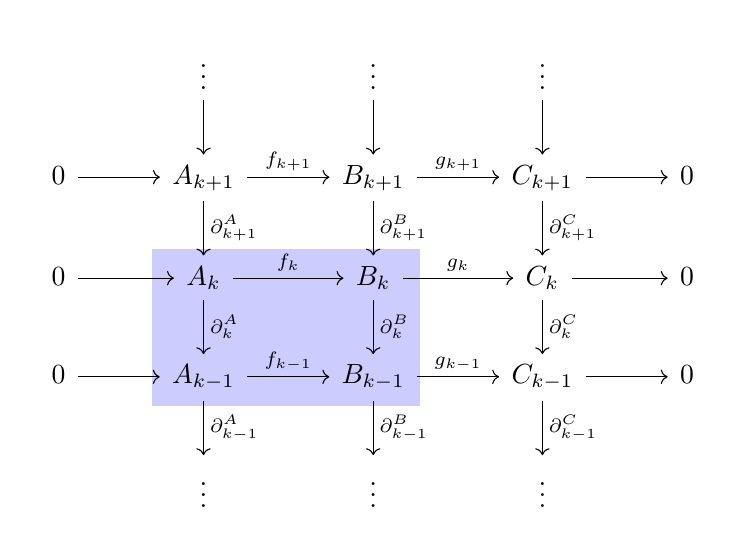
\begin{tikzpicture}
\usetikzlibrary{cd}


\fill[fill=blue!20]  (-2.8,3.2) rectangle (0.6,1.2);

\matrix[matrix of math nodes, name=m, commutative diagrams/every cell, row sep= 20, column sep = 30] {
\; & \vdots   & \vdots&\vdots &\\
0& A_{k+1} & B_{k+1} & C_{k+1}&0\\
0& A_{k} & B_{k} & C_{k}&0\\
0& A_{k-1} & B_{k-1} & C_{k-1}&0\\
\;&\vdots &\vdots &\vdots &\\};
\path[commutative diagrams/.cd, every arrow, every label]
(m-1-2) edge (m-2-2)    (m-1-3) edge (m-2-3)     (m-1-4) edge (m-2-4)
(m-2-1) edge (m-2-2)
(m-2-2) edge node {$\partial^A_{k+1}$} (m-3-2)    edge node {$f_{k+1}$} (m-2-3)      
(m-2-3)edge node {$\partial^B_{k+1}$} (m-3-3)    edge node {$g_{k+1}$}  (m-2-4)  
(m-2-4) edge node {$\partial^C_{k+1}$}(m-3-4)  edge (m-2-5)  

(m-3-1) edge (m-3-2)
(m-3-2) edge node {$\partial^A_{k}$} (m-4-2)    edge node {$f_{k}$} (m-3-3)      
(m-3-3)edge node {$\partial^B_{k}$} (m-4-3)    edge node {$g_{k}$}  (m-3-4)  
(m-3-4) edge node {$\partial^C_{k}$}(m-4-4)  edge (m-3-5)  

(m-4-1) edge (m-4-2)
(m-4-2) edge node {$\partial^A_{k-1}$} (m-5-2)    edge node {$f_{k-1}$} (m-4-3)      
(m-4-3)edge node {$\partial^B_{k-1}$} (m-5-3)    edge node {$g_{k-1}$}  (m-4-4)  
(m-4-4) edge node {$\partial^C_{k-1}$}(m-5-4)  edge (m-4-5)  
;
\end{tikzpicture}\]
\end{itemize}
This completes the proof that the map $\delta$ is well defined on homology. Now we will show some of the exactness statements. 
\begin{claim}
The sequence of homology groups 
\[H_k(B)\xrightarrow{g_k} H_k(C)\xrightarrow{\delta_k} H_{k-1}(A)\]
is exact. 
\end{claim}
In order to prove this claim, we need to show that $\ker(\delta)\subset \im(g_k)$, and $\im (g_k)\subset \ker \delta$. 
\begin{itemize}
\item To show that $\im(g_k)\subset \ker \delta$, it suffices to show that the composition $\delta_k \circ g_k=0$. Let $[\beta]\in H_k(B)$ be a homology class. Then $[\delta_k g_k(\beta)]= [f_{k-1}^{-1}(\partial^B_k\beta)]. $ Since $[\beta]$ is a class in homology, the boundary map starts by computing $\partial^B_k\beta=0$, and we conclude that $\delta_k (g_k(\beta))=0$. 
\item To show that the $\ker(\delta_k)\subset \im (g_k)$, let $\gamma$ be an element so that $\delta_k[\gamma]=0$. Since the map $g_k: B_k\to C_k$ is surjective, we might hope that $\beta=g^{-1}_k\gamma$, a choice of lift of $\gamma$, is a class in homology. So we need to show that $\partial^B_k(\beta)=0$. By commutativity of the lower right square, we have that 
$\partial^B_k(\beta)=f_{k-1}(\delta(\gamma))=0.$
\[ 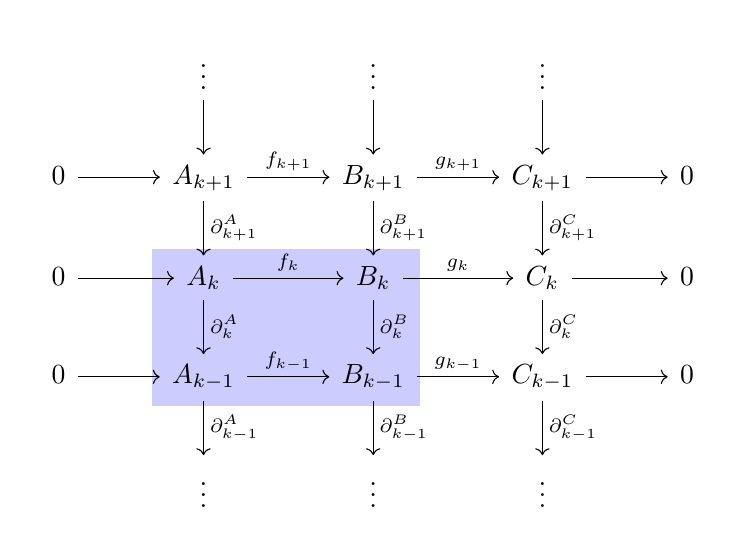
\begin{tikzpicture}
\usetikzlibrary{cd}


\fill[fill=blue!20]  (-2.8,3.2) rectangle (0.6,1.2);

\matrix[matrix of math nodes, name=m, commutative diagrams/every cell, row sep= 20, column sep = 30] {
\; & \vdots   & \vdots&\vdots &\\
0& A_{k+1} & B_{k+1} & C_{k+1}&0\\
0& A_{k} & B_{k} & C_{k}&0\\
0& A_{k-1} & B_{k-1} & C_{k-1}&0\\
\;&\vdots &\vdots &\vdots &\\};
\path[commutative diagrams/.cd, every arrow, every label]
(m-1-2) edge (m-2-2)    (m-1-3) edge (m-2-3)     (m-1-4) edge (m-2-4)
(m-2-1) edge (m-2-2)
(m-2-2) edge node {$\partial^A_{k+1}$} (m-3-2)    edge node {$f_{k+1}$} (m-2-3)      
(m-2-3)edge node {$\partial^B_{k+1}$} (m-3-3)    edge node {$g_{k+1}$}  (m-2-4)  
(m-2-4) edge node {$\partial^C_{k+1}$}(m-3-4)  edge (m-2-5)  

(m-3-1) edge (m-3-2)
(m-3-2) edge node {$\partial^A_{k}$} (m-4-2)    edge node {$f_{k}$} (m-3-3)      
(m-3-3)edge node {$\partial^B_{k}$} (m-4-3)    edge node {$g_{k}$}  (m-3-4)  
(m-3-4) edge node {$\partial^C_{k}$}(m-4-4)  edge (m-3-5)  

(m-4-1) edge (m-4-2)
(m-4-2) edge node {$\partial^A_{k-1}$} (m-5-2)    edge node {$f_{k-1}$} (m-4-3)      
(m-4-3)edge node {$\partial^B_{k-1}$} (m-5-3)    edge node {$g_{k-1}$}  (m-4-4)  
(m-4-4) edge node {$\partial^C_{k-1}$}(m-5-4)  edge (m-4-5)  
;
\end{tikzpicture}\]

\end{itemize}
\begin{claim}
The sequence of homology groups  
\[H_{k+1}(C)\xrightarrow{\delta_{k+1}} H_k(A)\xrightarrow{f_k} H_k(B)\]
is exact. 
\end{claim}
\end{proof}
\laststation{Exercises}

The zero vector space, $0$, is the vector space which only has one element in it. 
\begin{exercise}
	Let $V_1$ and $V_2$ be vector spaces.
	Suppose that $f: V_1\to V_2$ is a linear map. 
	Show that $\ker(f)=\{0\}$ if and only if the map $f: V_1\to V_2$ is injective.
\end{exercise}

\begin{exercise}Suppose we have 5 vectors spaces and maps between them. 
	\[
		\begin{tikzcd}
			V^0\arrow{r}{d^0} & V^1 \arrow{r}{d^1} & V^2\arrow{r}{d^2} & V^3 \arrow{r}{d^3} & V^4
		\end{tikzcd}
	\]
	and suppose that $\im d^i=\ker d^{i+1}$ for each $i$. 
	\begin{itemize}
		\item Show that $V^0=0$, then $d^1$ is injective. 
		\[\begin{tikzcd}
			0 \arrow{r}{d^0} & V^1 \arrow{r}{d^1} & V^2
		\end{tikzcd}
		\]
		\item Show that if $V^4=0$, then $d^2$ is surjective.
		\[\begin{tikzcd}
			V^2\arrow{r}{d^2} & V^3 \arrow{r}{d^3} & 0
		\end{tikzcd}
		\]
		\item Show that if $V^0=V^3=0$, then $d^1:V^1\to V^2$ is an isomorphism. 
		\[\begin{tikzcd}
			0\arrow{r}{d^0} & V^1 \arrow{r}{d^1} & V^2\arrow{r}{d^2} & 0
		\end{tikzcd}
		\]
		\item Show that if $V^0=V^4=0$, then $\dim(V^1)+\dim(V^3)=\dim(V^2)$. 
		\[
			\begin{tikzcd}
				0\arrow{r}{d^0} & V^1 \arrow{r}{d^1} & V^2\arrow{r}{d^2} & V^3 \arrow{r}{d^3} & 0
			\end{tikzcd}
		\]
		\item Furthermore, show that there is a non-canonical isomorphism of vector spaces, $V^2=V^1\oplus V^3$.
	\end{itemize}
	\end{exercise}
\begin{exercise}[Translating Sets in to Vector Spaces]
	Let $A$ be any finite set. Let $\mathcal F(A)$ be the set of functions $\phi: A\to \ZZ_2$. 
	\begin{itemize}
		\item Prove that there are $2^{|A|}$ such functions. 
		\item Prove that $\mathcal F(A)$ is a $\ZZ_2$ vector space. 
		\item Prove that $\dim(\mathcal F(A))=|A|$. 
	\end{itemize}
\end{exercise}
\begin{exercise}[Categories and Functors]
	Show that if $f: A\to B$ and $g: B\to C$ are two maps of sets, then 
	\[(g\circ f)^*=f^*\circ g^*,\]
	i.e. the pullback relation preserves compositions. 
\end{exercise}
\begin{exercise}
 Let $S_1, S_2 \subset A$ be two subsets as before. 
 
\[
	\begin{tikzcd}[row sep=4pt]
		\; & S_1 \arrow{dl}{i_1^*} \\
		S_1\cap S_2 &\oplus  & A\arrow{ul}{j_1^*} \arrow{dl}{j_2^*}\\
		\; & S_2\arrow{ul}{i_2^*}\\ \\ \\
		A^2 & A^1\arrow{l}{i^*} & A^0 \arrow{l}{j^*}
	\end{tikzcd}
\]
Prove that the map $i^*$ is surjective.
\end{exercise}
\begin{exercise}[Open Ended Exercise]
	Suppose that $S_1, S_2$ and $S_3$ are three sets, and $A=S_1\cup S_2\cup S_3$. Describe how one would extend the Inclusion-Exclusion formula to this setting using the linear algebra machinery that we set up before. 
\end{exercise}


\begin{exercise}
	Let $U\subset V$ be a subspace of a vector space. Consider the equivalence relation 
	\[v_1\sim_U v_2 \text{  if and only if  } v_1-v_2\in U.\]
	Show that the quotient space $V/U:=\{[v]_{\sim_U}\}$ given by the set of equivalence classes is a vector space.	
\end{exercise}
\begin{exercise}
	Let $U\subset V$ be a subspace of a vector space. Construct an exact chain complex
	\[0 \to U\to V\to V/U\to 0\]
\end{exercise}
\begin{exercise}
	Let $G$ be a graph -- a simplicial complex with only $0$ and $1$ dimensional simplices. The spaces $ C^0(G, \ZZ_2)$ and $ \underline C^1(G, \ZZ_2)$ have basis given by the vertices and edges of the graph. Describe $d^0$ as a matrix in terms of this basis. 
\end{exercise}
\begin{exercise}
	Show that whenever $e_1, \ldots, e_k$ sequence of edges with $k$ odd which form a cycle in $G$, then one of $e_1+\ldots+ e_k\in C^1(G, \ZZ_2)$ is not in the image of $d^0$. 
	Make a similar conclusion for when $k$ is even. 
	Conclude that if $G$ has a cycle, $\underline H^1(G):=H^1(\underline C^\bullet(G, \ZZ_2))$ is at least 1-dimensional.
\end{exercise}
\begin{exercise}
	Show that $\underline H^0(G)$ is one fewer than the number of connected components in $G$ . 
\end{exercise}
\begin{exercise}
	Show that $\underline H^1(G)=0$ if and only if $G$ is a tree. 
\end{exercise}
\begin{exercise}
	Suppose that $G$ has one connected component. Compute the dimension of $H^1(G)$ in terms of the number of edges and vertices of $G$.  
\end{exercise}
\begin{exercise}
	Let $S^2$ be the simplicial complex defined by the tetrahedron (do not include the interior 3-simplex, but only the 4 faces.) Show that $\underline H^0(S^2)=0, \underline H^2(S^2)=\ZZ_2$ and $H^1(S^2)=0$. 
\end{exercise}
\begin{exercise}
	Let $C^i(X, \ZZ_2)$ be the cochain complex associated to a simplicial space. Show that if $X$ has only one connected component then $\underline H^0(\ZZ_2)= 0$. 
\end{exercise}
In class, we looked at one configuration of open sets which covered the circle. We will look at some examples where we use multiple sets to cover a topological space. 
\begin{exercise}
    Let $X$ be the line segment drawn below, covered by two sets $U_1$ and $U_2$. Repeat the connected component construction for the line covered with two sets. 
    \[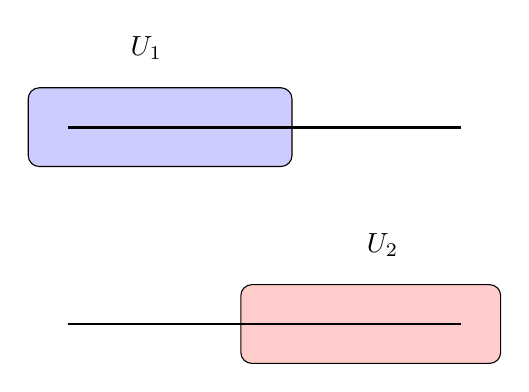
\begin{tikzpicture}

        \draw[rounded corners, fill=blue!20]  (-4,2) rectangle (-0.65,1);
        \draw[rounded corners, fill=red!20] (-1.3,-0.5) rectangle (2,-1.5);
        
        \draw[line width = 1pt] (-3.5,1.5) -- (1.5,1.5);
        \draw[line width = 1pt] (-3.5,-1) -- (1.5,-1);
        \node at (-2.5,2.5) {$U_1$};
        \node at (0.5,0) {$U_2$};
    \end{tikzpicture}\]
    Show that the map $i^*: C^1(X)\to C^2(X)$ is surjective, and so 
    \[ \dim(C^2(X))-\dim(\im(i^*))= \dim(\ker(0_{C^2(X)\to 0}))-\dim(\im(i^*))=0.\]
\end{exercise}
\begin{exercise}
    Let $X$ be the line segment, covered with $n$ open intervals which overlap as in the diagram below:
    \[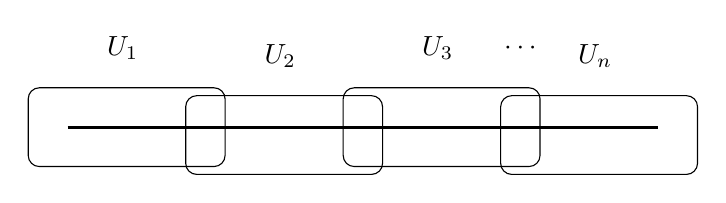
\begin{tikzpicture}

        \begin{scope}[]
        \draw[rounded corners]  (-4,2) rectangle (-1.5,1);
        \node at (-2.8,2.5) {$U_1$};
        \end{scope}\begin{scope}[shift={(4,0)}]
        \draw[rounded corners]  (-4,2) rectangle (-1.5,1);
        \node at (-2.8,2.5) {$U_3$};
        \end{scope}\begin{scope}[shift={(2,-0.1)}]
        \draw[rounded corners]  (-4,2) rectangle (-1.5,1);
        \node at (-2.8,2.5) {$U_2$};
        \end{scope}\begin{scope}[shift={(6,-0.1)}]
        \draw[rounded corners]  (-4,2) rectangle (-1.5,1);
        \node at (-2.8,2.5) {$U_n$};
        \end{scope}
        \draw[line width = 1pt] (-3.5,1.5) -- (4,1.5);
        \node at (2.25,2.5) {$\cdots$};
        \end{tikzpicture}
        \]
    Define a sequence 
    \[C^0(X)\xrightarrow{j^*}C^1(X)\xrightarrow{i^*}C^2(X)\]
    where $C^1(X)$ is based on the connected components of the $U_i$, and the $C^2(X)$ is based on the intersections $U_i\cap U_{i+1}$. 
    Again, show that 
    \[ \dim(C^2(X))-\dim(\im(i^*))= \dim(\ker(0_{C^2(X)\to 0}))-\dim(\im(i^*))=0.\]
\end{exercise}
\begin{exercise}
    Let $X$ be the circle, covered with $n$ intervals which overlap end to end as drawn below. 
    \[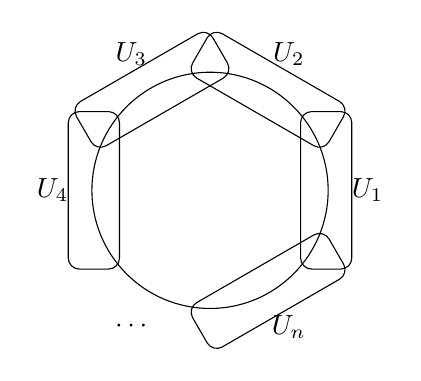
\begin{tikzpicture}
        \draw  (0,0) ellipse (1.5 and 1.5);
        \begin{scope}[]
        
        \draw[rounded corners]  (1.8,-1) rectangle (1.15,1);
        \node at (2,0) {$U_1$};
        \end{scope}
        \begin{scope}[rotate=60]
        
        \draw[rounded corners]  (1.8,-1) rectangle (1.15,1);
        \node at (2,0) {$U_2$};
        \end{scope}
        \begin{scope}[rotate=120]
        
        \draw[rounded corners]  (1.8,-1) rectangle (1.15,1);
        \node at (2,0) {$U_3$};
        \end{scope}
        \begin{scope}[rotate=180]
        
        \draw[rounded corners]  (1.8,-1) rectangle (1.15,1);
        \node at (2,0) {$U_4$};
        \end{scope}
        \begin{scope}[rotate=240]
        
        \node at (2,0) {$\cdots$};
        \end{scope}
        \begin{scope}[rotate=300]
        
        \draw[rounded corners]  (1.8,-1) rectangle (1.15,1);
        \node at (2,0) {$U_n$};
        \end{scope}
        \end{tikzpicture}\]
        Define $C^1(X)$ and $C^2(X)$ as in the previous problem.
        \begin{itemize}
        \item Pick a basis for $C^1(X)$ and $C^2(X)$ given by functions which map a single connected component to 1, and all other components to zero. Write down the map $i^*$ in this basis. 
        \item Show that for this cycle,
        \[ \dim(C^2(X))-\dim(\im(i^*))= \dim(\ker(0_{C^2(X)\to 0}))-\dim(\im(i^*))=-1.\]
        \end{itemize}
\end{exercise}
\begin{exercise}
    Cover this figure eight with sets so that
    \begin{itemize}
        \item Each set is connected 
        \item Each pair of sets intersect in one connected component
        \item No three sets have common overlap.
    \end{itemize}
\[    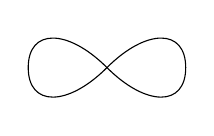
\begin{tikzpicture}
   \draw (-1,0.5) .. controls (-0.5,1) and (0,1) .. (0,0.5) .. controls (0,0) and (-0.5,0) .. (-1,0.5) .. controls (-1.5,1) and (-2,1) .. (-2,0.5) .. controls (-2,0) and (-1.5,0) .. (-1,0.5);
        \end{tikzpicture}\]
    Define a sequence 
    \[C^0(X)\xrightarrow{j^*}C^1(X)\xrightarrow{i^*}C^2(X)\]
    where $C^1(X)$ is based on the connected components of the $U_i$, and the $C^2(X)$ is based on intersection on the intersections $U_i\cap U_{k}$. 
    Then compute
    \[ \dim(\im(i^*))-\dim(C^2(X)).\]
\end{exercise}


\begin{exercise}
	Let $A^\bullet$ be a chain complex, and let $B^k:=H^k(A)$ be the chain complex whose cochain groups are given by the cohomology groups $H^k(A)$ and whose differential is always zero. 
	Verify that $\pi: A^\bullet\to B^\bullet$ which sends each element of $A$ to its cohomology class is a cochain map, and $\pi: H^k(A^\bullet)\to H^k(B^\bullet)$ is an isomorphism.
\end{exercise}
\begin{exercise}
	Let $X=(\Delta_X, \mathcal S_X)$ be a simplicial complex. A \emph{simplicial subcomplex} is a simplicial complex $Y=(\Delta_Y, \mathcal S_Y)$ with $\mathcal S_Y\subset \mathcal S_X$ and 
	\[\sigma\in \Delta_Y \Rightarrow \sigma\in \Delta_X.\]
	Show that if $Y$ is a subcomplex of $X$, there is a cochain map \[i^*: \underline C^\bullet(X, \ZZ_2)\to \underline C^\bullet(Y, \ZZ_2).\]
\end{exercise}
\begin{exercise}
	Let $Y\subset X$ be a simplicial subcomplex. 
	Denote the corresponding map of topological spaces $i: Y\to X$.
	Construct a new simplicial complex, $\cone(i)$ whose vertex set is  \[\mathcal S_{\cone}:= \mathcal S\cup\{x\},\]
	and whose simplifies are:
	\[\Delta_{\cone}:=\Delta_X\cup\{\sigma\cup\{x\}\;|\; \sigma \in \Delta_Y\}.\]
	Draw a picture for $\cone(i)$ when $X$ is an interval, and $Y$ is the two boundary vertices of the interval. 
	Furthermore, explain why this operation is called the cone.
\end{exercise}
\begin{exercise}
	Let $i^*:\underline C^\bullet(X, \ZZ_2)\to \underline C^\bullet(Y, \ZZ_2)$ be the map considered above. Prove that \[\underline C^\bullet(\cone(i), \ZZ_2 )=\cone^\bullet(i^*)[-1]\]
\end{exercise}
\begin{exercise}
	The $n$-disk  (denoted $D^n$) is the simplicial complex where $\mathcal S_{D^k}:=\{0, \ldots, n\}$ and 
	\[\Delta_{D^n}=\{\sigma \;|\; \sigma\subset \mathcal S_{D^n}\}.\]
	Let $\id_{D^n}: D^n\to D^n$ be the inclusion of $D^k$ into itself as a subcomplex. Show that 
	\[\cone(\id_{D^n})=D^{n+1}.\]
\end{exercise}
When $X$ is a simplicial complex, we denote by $H^i(X, \ZZ_2)$ to be the $i$-th cohomology group of $\underline C^\bullet(X, \ZZ_2)$.
\begin{exercise}
	Use the previous characterization of $D^{n+1}$ to compute the homology groups $\underline H^i(D^k)$ inductively. 
\end{exercise}
\begin{exercise}
	The $n$-sphere (denoted $S^n$) is the simplicial complex where ${\mathcal S}_{S^n}=\{0, \ldots, n+1\}$ and 
	\[\Delta_{S^n}=\{\sigma \;|\; \sigma\subset {\mathcal S}_{S^n}, \sigma \neq \{0, \ldots, n+1\}.\]
	Show that there is a map $i_{S^n}: S^n\to D^{n+1}$, and that 
	\[\cone(i_{S^n})=S^{n+1}.\]
\end{exercise}
\begin{exercise}
	Use the previous characterization of $S^{n+1}$ to compute the cohomology groups $\underline H^i(S^n)$ inductively. 
\end{exercise}

